\documentclass[10pt]{article}

% DOCUMENT LAYOUT
%\usepackage{fullpage}
%\usepackage[cm]{fullpage}
%\usepackage[letterpaper, top=0.5in, bottom=0.5in, left=0.5in, right=0.5in]{geometry} 
%\usepackage[letterpaper]{geometry} 
%\geometry{textwidth=5.7in, textheight=9.0in, marginparsep=7pt, marginparwidth=.6in}
%\geometry{textwidth=6.0in, textheight=9.8in, marginparsep=7pt, marginparwidth=.8in}
%\geometry{textwidth=6in, textheight=9.8in, marginparsep=7pt, marginparwidth=.8in}
\setlength\parindent{0in}

% Dynamically control baselinestretch
\usepackage{setspace}

% Local hyphenation control
\usepackage{hyphenat}

% highlighting
\usepackage{color,soul}

%\addtolength{\oddsidemargin}{-.500in}
%\addtolength{\evensidemargin}{-.500in}
%\addtolength{\textwidth}{2.00in}

%\addtolength{\topmargin}{-.875in}
%\addtolength{\textheight}{1.75in}

\addtolength{\topmargin}{-1.125in}
\addtolength{\textheight}{2.0in}

\addtolength{\oddsidemargin}{-.375in}
\addtolength{\evensidemargin}{-.375in}
\addtolength{\textwidth}{1.75in}
\addtolength{\marginparsep}{-10pt}
\addtolength{\marginparwidth}{+15pt}

\usepackage{wrapfig}

\usepackage{chngpage}
\usepackage[export]{adjustbox}

\usepackage{sidecap}
\usepackage[abs]{overpic}
\usepackage{wrapfig}

% SPECIAL FORMATTING
% ---- CUSTOM AMPERSAND
\newcommand{\amper}{{\selectfont\itshape\&}}
% ---- MARGIN YEARS
%\newcommand{\years}[1]{\marginpar{\scriptsize #1}}
\newcommand{\years}[1]{\marginpar{\quad \small #1}}
% ---- TALK COUNTER
\newcounter{talknumber}
\setcounter{talknumber}{1}
% ---- ARTICLE COUNTER
\newcounter{articlenumber}
\setcounter{articlenumber}{1}
%\newcommand{\article}{\noindent\marginpar{\scriptsize \arabic{articlenumber}}\addtocounter{articlenumber}{1}}
\newcommand{\article}[2]{
\noindent\marginpar{
  \parbox[c]{0.25in}{\scriptsize \arabic{articlenumber}} 
  \parbox[c]{0.25in}{\scriptsize \href{#2}{#1}}
}\addtocounter{articlenumber}{1}}
% PAPER DESCRIPTION AND THUMBNAIL IMAGE
\newcommand{\desc}[2]{
\noindent\marginpar{
  \parbox[c]{0.50in}{{\includegraphics[width=0.9in]{thumbnails/{#1}}}}
}{\footnotesize\emph{#2}}}
% NEW ARTICLE STYLE WITH IMAGE AND NO NUMBERS
% #1 : thumbnail filename
% #2 : author list
% #3 : article title
% #4 : journal reference
% #5 : DOI, bioR$\chi$v, or ar$\chi$iv
% #6 : DOI, bioR$\chi$v, or arXiv link
% #7 : blurb / description
\newcommand{\newarticle}[7]{
\begin{adjustwidth}{-1in}{-1in}  
\begin{tabular}{p{0.9in}p{7in}}
%\parbox[c]{0.9in}{\includegraphics[width=0.9in]{thumbnails/{#1}}} & \parbox[c]{6in}{\setstretch{0.9} {\small #4} $\cdot$ \href{#6}{#5} \\ {\scriptsize {#2}} \\ \raggedright { \bf\nohyphens{#3}}  \\ {\footnotesize\emph {#7}}} % authors too small
\parbox[c]{0.9in}{\includegraphics[width=0.9in]{thumbnails/{#1}}} & \parbox[c]{6in}{\setstretch{0.9} {\small #4} $\cdot$ \href{#6}{#5} \\ {\footnotesize {#2}} \\ \raggedright { \bf\nohyphens{#3}}  \\ {\footnotesize\emph {#7}}}
\end{tabular}
\end{adjustwidth}
\vspace{0.2in}
}

% ---- TALKS
\newcommand{\talk}[2]{
\noindent\marginpar{
   \scriptsize \scshape
  #2 \\ #1
}}
\newcommand{\numberedtalk}[2]{
\noindent\marginpar{
  \parbox[c]{0.25in}{\scriptsize \arabic{talknumber}} 
% \parbox[c]{0.5in}{\scriptsize {#2}}
  \parbox[c]{0.5in}{\scriptsize \scshape {#1}}
}\addtocounter{talknumber}{1}}

\newcommand{\newtalk}[3]{
\noindent\marginpar{
   \scriptsize \scshape
  #2 \\ #1
}\spaceTalk\\}

% SPACING
\newcommand{\spaceEd}{\vspace{1ex}}
\newcommand{\spaceRes}{\vspace{1ex}}
\newcommand{\spaceFell}{\vspace{0.5ex}}
\newcommand{\spacePub}{\vspace{0.5ex}}
\newcommand{\spaceTalk}{\vspace{1ex}}
\newcommand{\spaceSoc}{\vspace{0.5ex}}
\newcommand{\spacePost}{\vspace{0.5ex}}

\newcommand{\jdc}{ {\bf \hl{Chodera~JD}} } % highlight
%\newcommand{\jdc}{\underline{\bf Chodera~JD}} % underline

% Modify section spacing
%\usepackage{titlesec}
%\titlespacing*{\section}{0pt}{0.2\baselineskip}{\baselineskip}
%\titlespacing*{\subsection}{0pt}{0.2\baselineskip}{\baselineskip}
%\titlespacing*{\subsubsection}{0pt}{0.2\baselineskip}{\baselineskip}

% GRAPHICS
\usepackage{graphicx}

% HEADINGS
\usepackage{sectsty} 
\usepackage[normalem]{ulem} 

\usepackage{fancyhdr}
\renewcommand{\headrulewidth}{0pt}
\pagestyle{fancy}
\fancyhf{}
%\fancyfoot[LE,CO]{{\small\textsc{John D. Chodera - Sloan Kettering Institute - \thepage}}}%
\rfoot{\small\textsc{John D. Chodera - Sloan Kettering Institute - \thepage}}

% Clean up font spacing with micro type
\usepackage{microtype}

% Use a clean, modern-looking font
\usepackage[default]{lato}
%\usepackage[default]{raleway}
%\usepackage{avant}
%\renewcommand*\familydefault{\sfdefault} %% Only if the base font of the document is to be sans serif
%\usepackage[sfdefault,light]{roboto}  %% Option 'sfdefault' only if the base font of the document is to be sans serif
\usepackage[T1]{fontenc}

% Change the appearance of section and subsection headings
\sectionfont{\mdseries\large\underline} 
\subsectionfont{\mdseries\scshape\normalsize} 
\subsubsectionfont{\bfseries\upshape\normalsize} 

% Control tightness of spacing
\renewcommand{\baselinestretch}{1.1}

% PDF SETUP
% ---- FILL IN HERE THE DOC TITLE AND AUTHOR
\usepackage[bookmarks, colorlinks, breaklinks, pdftitle={John D. Chodera - vita},pdfauthor={John D. Chodera}]{hyperref}  
\hypersetup{linkcolor=blue,citecolor=blue,filecolor=black,urlcolor=blue} 

% Change the typewriter font to something nicer.
\usepackage[ttdefault]{sourcecodepro}

% DOCUMENT
\begin{document}
\reversemarginpar
% FILL IN NAME HERE
{\fontseries{eb}\selectfont \LARGE John D. Chodera}\\[1cm]

% FILL IN AUTHOR INFORMATION HERE
\begin{minipage}[t]{2.5in}
%
\includegraphics[width=0.7in,valign=c]{images/john_chodera_sm.pdf}
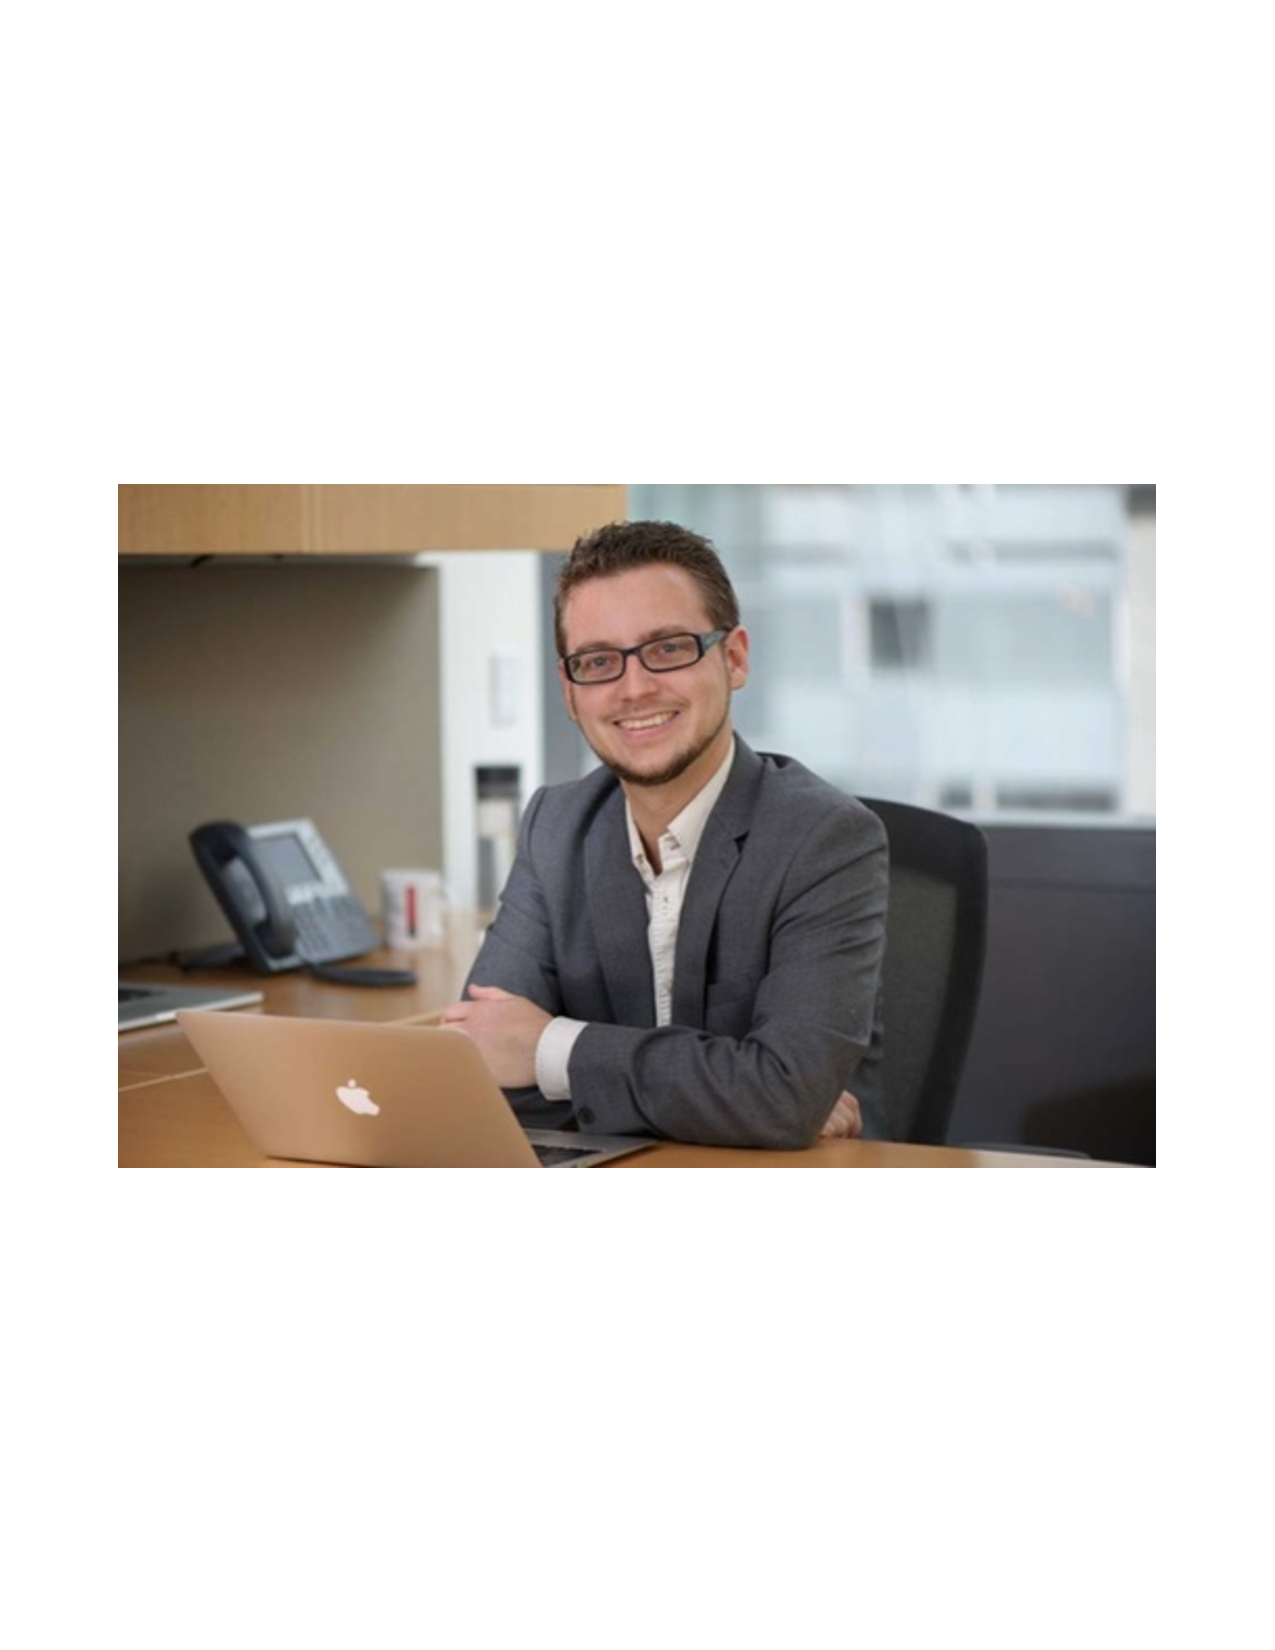
\includegraphics[width=2.5in,valign=c]{images/john_chodera_wide.pdf}
\end{minipage}
\quad
\begin{minipage}[t]{3in}
\begin{tabular}{rl}
{\bf url} & \href{http://www.choderalab.org}{http://www.choderalab.org}\\[0.05in]
{\bf email} & \href{mailto:choderaj@mskcc.org}{\href{mailto:john.chodera@choderalab.org}{john.chodera@choderalab.org}}\\[0.05in]
{\bf github} & \href{https://github.com/choderalab}{https://github.com/choderalab}\\[0.05in]
{\bf ORCID iD} & \href{http://orcid.org/0000-0003-0542-119X}{0000-0003-0542-119X}\\[0.05in]
{\bf twitter} & \href{http://twitter.com/jchodera}{@jchodera}\\[0.05in]
{\bf mobile} & 415.867.7384\\[0.05in]
%{\bf fax} & 646.422.0717 \\[0.05in]
%{\bf mobile} & 646.737.3319\\[0.05in]
{\bf post} & 
\parbox[t]{3.0in}{%Memorial Sloan Kettering Cancer Center\\
1275 York Ave, Box 357\\
New York, NY 10065}
\end{tabular}
\end{minipage}

% RESEARCH INTERESTS
%\section*{Research interests}
%\noindent {\bf Computational biophysics}, especially \\
%\noindent {\bf Single-molecule biophysics}, including new techniques for interpreting force microscopy \\
%\noindent {\bf Nonequilibrium statistical mechanics}, as tools for single-molecule experimental probes and the design of new algorithms for computational chemistry \\



\setstretch{1.05} 

\vspace{-0.15in}
\section*{Education and positions}
\vspace{-0.15in}

\noindent\years{2013--}{\bf Assistant Professor, Physiology, Biophysics, and Systems Biology Program,\\
Weill Cornell Graduate School of Medical Sciences}\\
\noindent\years{2012--}{\bf Assistant Member, Memorial Sloan-Kettering Cancer Center}\\
\noindent\years{2008--2012}{\bf Independent Distinguished Postdoctoral Fellow, California Institute for Quantitative Biosciences (QB3),\\
University of California, Berkeley}\\
Independent research funding, sponsors \href{http://www.cchem.berkeley.edu/plggrp/index.html}{Phillip L. Geissler} and \href{http://zebra.berkeley.edu/}{Susan Marqusee} \\
%\noindent\years{2011--2012}{\bf \href{http://research.google.com/university/exacycle_program.html}{Google Exacycle Visiting Faculty}} \\
\noindent\years{2006--2008}{\bf Postdoctoral researcher, Department of Chemistry, Stanford University}\\
With \href{https://pande.stanford.edu/}{Vijay S. Pande} (head of \href{http://folding.stanford.edu}{Folding@Home} distributed computing project) \\
\noindent\years{1999--2006}{\bf \textsc{Ph.D.} in Biophysics, University of California, San Francisco}\\
%Dissertation: \href{http://www.dillgroup.ucsf.edu/~jchodera/pubs/pdf/jdcthesis.pdf}{\emph{Master equation models of macromolecular dynamics from atomistic simulation.}} \\
Committee: \href{http://www.dillgroup.org}{Ken A. Dill}, \href{http://jacobsonlab.org/}{Matthew P. Jacobson}, \href{https://pande.stanford.edu/}{Vijay S. Pande}\\
\noindent\years{1995--1999}{\bf \textsc{B.S.} in Biology, California Institute of Technology}\\
Undergraduate research with \href{http://www.its.caltech.edu/~phplab/phplab.html}{Paul H.~Patterson} (\emph{experimental molecular neurobiology}) \\and Jerry E.~Solomon (\emph{computational chemistry})

\vspace{-0.15in}
\section*{Fellowships and awards}
\vspace{-0.15in}

\noindent\years{2017}Silicon Therapeutics Open Science Fellowship\\
\noindent\years{2013--2016}Louis V.~Gerstner Young Investigator Award\\
\noindent\years{2013--2014}Google Exacycle for External Faculty\\
\noindent\years{2008--2012}QB3-Berkeley Distinguished Postdoctoral Fellowship, University of California, Berkeley\\
%\noindent\years{2008}Berkeley Mini Stat Mech Meeting Best Poster Prize (second place)\\
\noindent\years{2005--2006}IBM Predoctoral Fellowship\\
\noindent\years{2005}Frank M. Goyan Award for outstanding work in physical chemistry, University of California, San Francisco\\
\noindent\years{2000--2005}Howard Hughes Medical Institute Predoctoral Fellowship
%\noindent\years{1998--1999}Caltech Upperclass Merit Award Scholarship\\
%\noindent\years{1997,$\:$1998}Caltech Summer Undergraduate Research Fellowships


\vspace{-0.15in}
\section*{Research overview}
\vspace{-0.15in}

%\noindent{Rational computational design of allosteric small-molecule inhibitors and therapeutics}\\
%\noindent{Kinase inhibitor selectivity and evolution of therapeutic resistance in cancer}\\
%\noindent{Biomolecular dynamics and conformational heterogeneity}\\
%\noindent{Error and uncertainty in biophysical measurements}\\
%\noindent{Computational chemistry, molecular modeling, and forcefield development}\\
%\noindent{Multiscale modeling of the effects of small molecules on biochemical pathways}

%My research focuses on the use of rigorous statistical mechanics, physical modeling, and statistical inference to develop quantitative, predictive computational models to enable the engineering of small molecules with desired properties. At the Sloan Kettering Institute, my laboratory consists of twelve theorists and experimentalists that combine theory, advanced simulation algorithms, high performance computing, and automated biophysical measurements to develop quantitative models for the design of small molecules. My laboratory has extensive experience in the use of atomistic molecular simulation, physical modeling, alchemical free energy calculations for the computation of free energies of transfer, and physical cheminformatics. We heavy use of large-scale computational resources, including the Folding@home distributed computing platform, national supercomputing resources, and high-performance GPU computing resources at MSKCC. Our laboratory also has extensive experience with statistical inference methods and techniques for experimental design guided by Bayesian inference and information theoretic principles, as well as the use of Bayesian inference and bootstrap simulation for accurate assessment of measurement error.

%{\bf My laboratory at MSKCC uses computation and automated biophysical experiments to develop new algorithms and approaches to the rational design of small molecules that selectively modulate cellular pathways.}
%We develop new GPU-accelerated algorithms for alchemical free energy calculations~\cite{tembe-mccammon:comput-chem:1984:alchemical-free-energy-calculations,shirts-mobley-chodera:2007:annu-rep-comput-chem:prime-time,chodera:curr-opin-struct-biol:2011:drug-discovery,wang:jcamd:2013:yank} in order to predict and optimize the affinity and selectivity of small molecules for their intended biomolecular targets.
%We have designed and built an automated biophysical wetlab to test these predictions, study the evolution of mutational resistance in targeted kinase inhibitors, and refine computational algorithms and forcefields.
%In addition, we employ the Folding@home worldwide distributed computing platform---where hundreds of thousands of donors around the world contribute their computing power~\cite{shirts-pande:science:2000:folding-at-home,folding-at-home-stats}---to study the conformational dynamics of cancer targets (such as kinases, small GTPases like Ras, and protein methyltransferases) in order to understand function, disease, and opportunities for allosteric modulation with small molecules.
%Major collaborations with both academic laboratories and pharmaceutical companies use computation and biophysical experiment to explore various aspects of biomolecular dynamics, drug pharmacokinetics, design of biological therapeutics, new biophysical measurement and screening technologies, and emerging targets.

My research focuses on {\bf redesigning the way we develop small molecules for chemical biology and drug discovery} and {\bf bringing rigorous atomistic modeling into the high-throughput biology and genomics era}.
By combining novel algorithmic advances to achieve orders-of-magnitude efficiency gains with powerful but inexpensive GPU hardware and distributed computing technologies, I am developing a new generation of tools and open source software packages for predicting small molecule binding affinities, designing small molecules with desired properties, quantifying drug sensitivity or resistance of clinical mutations, and understanding the detailed structural mechanisms underlying oncogenic mutations.
As a core member of the \href{https://foldingathome.stanford.edu/about/the-foldinghome-consortium/}{Folding@home Consortium}, my lab harnesses the computing power of hundreds of thousands of volunteers around the world to study functional implications of mutations and new opportunities for therapeutic design against cancer targets.
Using automated biophysical measurements, we collect new experimental data targeted to advance the quantitative accuracy of our methodologies, and gather new insight into drug susceptibility and resistance in kinases and other cancer targets.
My work makes extensive use of scalable Bayesian statistical inference methods and information theoretic principles for designing experiments and quantifying error.
I am passionate about open science, disseminating software engineering best practices, and maximizing research reproducibility.

\setstretch{1.00} 

\eject

%%%%%%%%%%%%%%%%%%%%%%%%%%%%%%%%%%%%%%%%%%%%%%%%%%%%%%%%%%%%%%%%%%%%%%%%%%%%%%%%
% PUBLICATIONS
%%%%%%%%%%%%%%%%%%%%%%%%%%%%%%%%%%%%%%%%%%%%%%%%%%%%%%%%%%%%%%%%%%%%%%%%%%%%%%%%

\section*{Publications}

\setstretch{1.05} 

\begin{minipage}[t]{3in}
Google Scholar statistics: \href{http://goo.gl/qO0JW}{http://goo.gl/qO0JW} \hspace{0.2in} \\
MyNCBI Bibliography: \href{http://goo.gl/e3kjgK}{http://goo.gl/e3kjgK} \\
{\small \it h-index: 38 / i10-index: 54 / citations: 7698 (3 Sep 2018)} \\
{\scriptsize $^*$ denotes co-first-authors \\
$\dag$ denotes co-second-authors \\
$\ddag$ denotes co-corresponding authors}
\end{minipage}
\quad
\begin{minipage}[t]{3in}
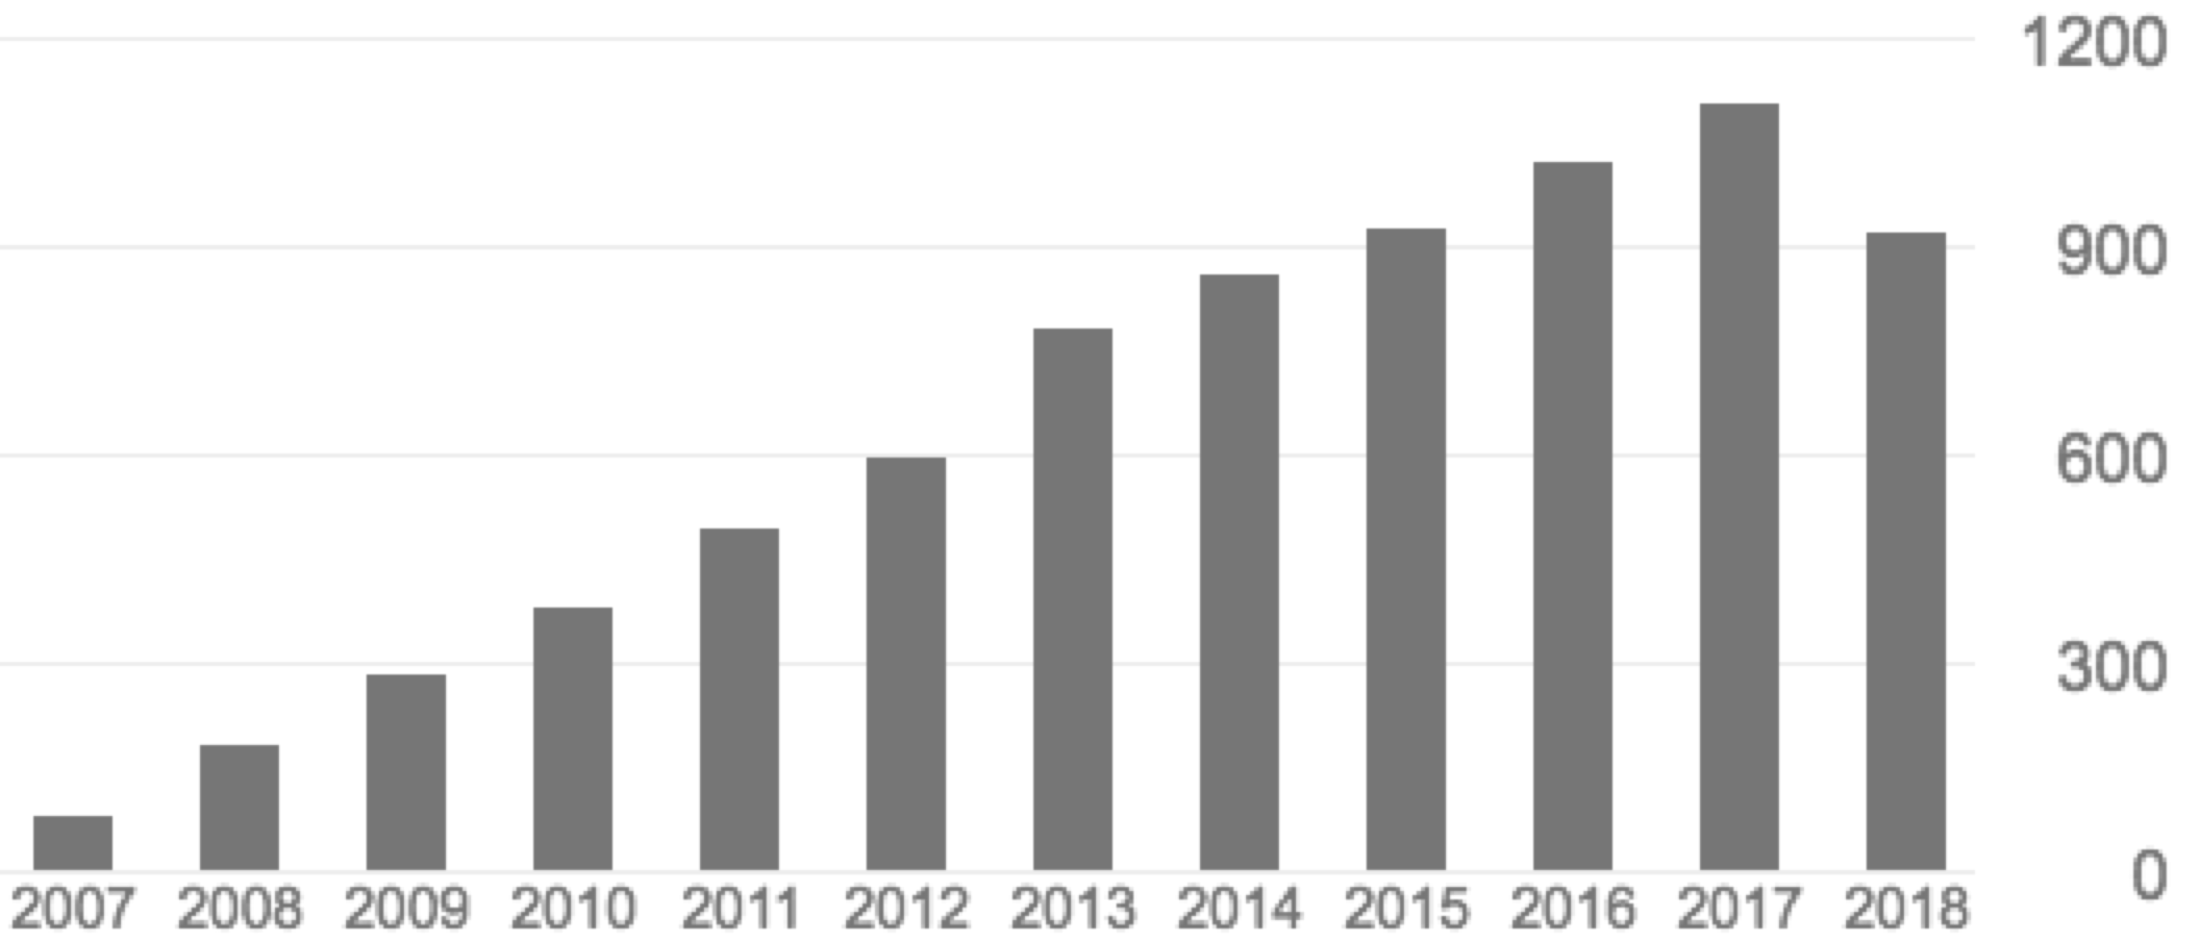
\includegraphics[width=3in,valign=c]{thumbnails/citations-2018-09-03.png}

\vspace{0.05in}
{\small annual citation counts (Google Scholar) -- 3 Sep 2018}
\end{minipage}

\setstretch{1.00} 

%%%%%%%%%%%%

\section*{Submitted and Under Review}

\newarticle{id1}{Paulina M. Wojnarowicz, Raquel Lima e Silva, Masayuki Ohanka, Sang Bae Lee, Yvette Chin, Anita Kulukian, Sung-Hee Chang, Bina Desai, Marta Garcia Escolano, Riddhi Shah, Marta Garcia-Cao, Sijia Xu, Rashmi Thakar, Yehuda Goldgur, Meredith A. Miller, Ouathek Ouerfelli, Guangli Yang, Tsutomu Arakawa, Steven K. Albanese, William A. Garland, Glenn Stoller, Jaideep Chaudhary, Rajesh Soni, John Philip, Ronald C. Hendrickson, Antonio Iavarone, Andrew J. Dannenberg, \jdc, Nikola Pavletich, Anna Lasorella, Peter A. Campochiaro, and Robert Benezra}{A novel small-molecule pan-Id antagonist inhibits pathologic ocular neovascularization}{Submitted}{}{}{We report the discovery and characterization of a small molecule, AGX51, with the surprising ability to inhibit the interaction of Id1 with E47, which leads to ubiquitin-mediated degradation of Ids.}

\newarticle{setd8-msm}{Rafal P. Wiewiora$^\dag$, Shi Chen$^\dag$, Fanwang Meng, Nicolas Babault, Anqi Ma, Wenyu Yu, Kun Qian, Hao Hu, Hua Zou, Junyi Wang, Shijie Fan, Gil Blum, Fabio Pittella-Silva, Kyle A. Beauchamp, Wolfram Tempel, Hualing Jiang, Kaixian Chen, Robert Skene, Y. George Zheng, Peter J. Brown, Jian Jin, \jdc$^\ddag$, and Minkui Luo$^\ddag$}{The dynamic conformational landscapes of the protein methyltransferase SETD8}{Submitted}{}{}{In this work, we show how targeted X-ray crystallography using covalent inhibitors and depletion of native ligands to reveal structures of low-population hidden conformations can be combined with massively distributed molecular simulation to resolve the functional dynamic landscape of the protein methyltransferase SETD8 in unprecedented atomistic detail. Using an aggregate of six milliseconds of fully atomistic simulation from Folding\@home, we use Markov state models to illuminate the conformational dynamics of this important epigenetic protein.}

\newarticle{ddr1-dfg-pmf}{Hanson SM$^*$, Georghiou G$^*$, Miller WT, Rest JS, \jdc, and Seeliger MA}{What makes a kinase promiscuous for inhibitors?}{Submitted}{}{}{Using a combination of chemogenomics, structural biology, and molecular simulation approaches, we identify a set of human kinases that are especially promiscuous binders of small molecule kinase inhibitors, and show that a prototypical member of this class, DDR1, achieves this promiscuity by virtue of its more stable Asp-DFG-out conformation.}

\newarticle{sampl6-host-guest-overview}{Rizzi A, Murkli S, McNeill J, Yao W, Sullivan M, Gilson MK, Chiu MW, Isaacs L, Gibb BC, Mobley DL$\ddag$, and \jdc$\ddag$}{Overview of the SAMPL6 host-guest binding affinity prediction challenge}{Submitted}{bioRiv}{https://doi.org/10.1101/371724}{We present an overview of the host-guest systems and participant performance for the SAMPL6 host-guest blind affinity prediction challenges, assessing how well various physical modeling approaches were able to predict ligand binding affinities for simple ligand recognition problems where receptor sampling and protonation state effects are eliminated due to the simplicity of supramolecular hosts. We find that progress is now stagnated likely due to force field limitations.}

\newarticle{sampl6-pka-measurements}{Isik M, Levorse D, Rustenburg AS, Ndukwe IE, Wang H, Reibarkh M, Martin GE, Makarov AA, Mobley DL, Rhodes T$\ddag$, and \jdc$\ddag$}{pKa measurements for the SAMPL6 prediction challenge for a set of kinase inhibitor-like fragments}{Submitted}{bioRxiv}{http://biorxiv.org/cgi/content/short/368787v1}{The SAMPL5 blind challenge exercises identified neglect of protonation state effects as a major accuracy-limiting factor in physical modeling of biomolecular interactions. In this study, we report the experimental measurements behind a SAMPL6 blind challenges in which we assess the ability of community codes to predict small molecule pKas for small molecule resembling fragments of selective kinase inhibitors.}

\newarticle{smirnoff}{Mobley DL$\ddag$, Bannan CC, Rizzi A, Bayly CI, \jdc, Lim VT, Lim NM, Beauchamp KA, Shirts MR, Gilson MK, and Eastman PK}{Escaping atom types using direct chemical perception with SMIRNOFF v0.1}{Submitted}{bioRxiv}{https://doi.org/10.1101/286542}{We describe the philosophy behind a modern approach to molecular mechanics forcefield parameterization, and present initial results for the first SMIRNOFF-encoded forcefield: SMIRNOFF99Frosst.}

\newarticle{smarty}{Zanette C, Bannan CC, Bayly CI, Fass J, Gilson MK, Shirts MR, \jdc, Mobley DL$\ddag$}{Toward learned chemical perception of force field typing rules}{Submitted}{chemRxiv}{https://chemrxiv.org/articles/Toward_Learned_Chemical_Perception_of_Force_Field_Typing_Rules/6230627}{We show how machine learning can learn typing rules for molecular mechanics force fields within a Bayesian statistical framework.}

\newarticle{bayesian-itc}{Nguyen TH, Rustenburg AS, Krimmer SG, Zhang H, Clark JD, Novick PA, Branson K, Pande VS, \jdc$\ddag$, MinH DDL$\ddag$}{Bayesian analysis of isothermal titration calorimetry for binding thermodynamics}{Submitted}{bioRxiv}{https://doi.org/10.1101/327676}{We show how Bayesian inference can produce greatly improved estimates of statistical uncertainty from isothermal titration calorimetry (ITC) experiments, allowing the joint distribution of thermodynamic parameter uncertainties to be inferred.}

\newarticle{musashi}{Minuesa G, Albanese SK, Chow A, Schurer A, Park SM, Rotsides CZ, Taggart J, Rizzi A, Naden LN, Chou T, Gourkanti S, Cappel D, Passarelli MC, Fairchild L, Adura C, Glickman FJ, Schulman J, Famulare C, Patel M, Eibl JK, Ross GM, Tan DS, Leslie CS, Beeming T, Golgur Y, \jdc, and Kharas MG. }{Small-molecule targeting of MUSASHI RNA-binding activity in acute myeloid leukemia}{Submitted}{bioRxiv}{https://doi.org/10.1101/321174}{We use absolute alchemical free energy calculations to identify the likely interaction site for a small hydrophobic ligand that shows activity against MUSASHI in AML.}

\newarticle{ops}{Swenson DWH, Prinz JH, No\'{e} F, \jdc, and Bolhuis PG}{OpenPathSampling: A Python framework for path sampling simulations. I. Basics}{Submitted}{bioRxiv}{https://doi.org/10.1101/351494}{To make powerful path sampling techniques broadly accessible and efficient, we have produced a new Python framework for easily implementing path sampling strategies (such as transition path and interface sampling) in Python. This first publication describes some of the theory and capabilities behind the approach.}

\newarticle{ops}{Swenson DWH, Prinz JH, No\'{e} F, \jdc, and Bolhuis PG}{OpenPathSampling: A Python framework for path sampling simulations. II. Building and customizing path ensembles and sample schemes}{Submitted}{bioRxiv}{https://doi.org/10.1101/351510}{To make powerful path sampling techniques broadly accessible and efficient, we have produced a new Python framework for easily implementing path sampling strategies (such as transition path and interface sampling) in Python. This second publication describes advanced aspects of the theory and details of how to customize path ensembles.}

%\newarticle{id1}{Wojnarowicz P, Desai B, Chin Y, Lima e Silva R, Ohnaka M, Lee SB, Cao MG, Ouerfelli O, Xu S, Goldgur Y, Miller M, Chaudhary J, Garland W, Stoller G, Albanese SA, Soni R, Philip J, Healey J, Vinagolu R, Norton L, Rosen N, Hendrickson R, Iavarone A, Dannenberg A, \jdc, Pavletich N, Lasorella A, Campochiaro P, Benezra R}{A small-molecule pan Id antagonist, AGX51, shows strong anti-tumor and anti-neovascular activity}{In revision}{bioR$\chi$iv}{https://doi.org/10.1101/205260}{We identify the binding mode of a new small-molecule pan-Id antagonist prior to its confirmation by mass spectrometry crosslinking data.}

%\eject

%%%%%%%%%%%%

\subsection*{Published and In Press}

\newarticle{kinase-mutations}{Hauser K, Negron C, Albanese SK, Ray S, Steinbrecher T, Abel R, and \jdc, and Wang L}{Predicting resistance of clinical Abl mutations to targeted kinase inhibitors using alchemical free-energy calculations}{\emph{Communications Biology} 1:70, 2018}{DOI}{https://doi.org/10.1038/s42003-018-0075-x}{We show how alchemical free energy calculations can be used to predict whether clinical point mutations in human kinase domains confer resistance or susceptibility to targeted kinase inhibitors.}

\newarticle{kinome-expression-tree}{Albanese SK*, Parton DL*, Isik M$\dag$, Rodr\'{i}guez-Laureano L$\dag$, Hanson SM, Gradia S, Jeans C, Levinson NM, Seeliger M, and \jdc}{An open library of human kinase domain constructs for automated bacterial expression}{\emph{Biochemistry} 57:4675, 2018}{DOI}{http://doi.org/10.1021/acs.biochem.7b01081}{To establish a tractable experimental system for studying the biophysical determinants of selective kinase inhibitor resistance in clinical cancer mutations, we engineer a library of human kinase domains with useful bacterial expression with phosphatase coexpression.}

\newarticle{idh2-trans-mutations}{Intlekofer AM*, Shih AH*, Wang B, Nazir A, Rustenburg AS, Albanese SK, Patel M, Famulare C, Correa FM, Arcila ME, Taylor J, Tallman MS, Roshal M,  Petsko GA, \jdc, Thompson CB$\ddag$, Levine RL$\ddag$, Stein, EM$\ddag$}{Acquired resistance to IDH inhibition through trans or cis dimer-interface mutations}{\emph{Nature} 559:125, 2018}{DOI}{https://doi.org/10.1038/s41586-018-0251-7}{Clinical double mutations acting in trans in cancer patients receiving IDH2 inhibitors act through a novel biophysical mechanism.}

\newarticle{configuration-space-error}{Fass J, Sivak DA, Crooks GE, Beauchamp KA, Leimkuhler B, and \jdc}{Quantifying configuration-sampling error in Langvevin simulations of complex molecular systems}{\emph{Entropy} 20:318, 2018}{DOI}{https://doi.org/10.3390/e20050318}{We address a fundamental question regarding why molecular dynamics simulation works despite the fact that the use of finite timesteps leads to error in the sampled probability densities and populations, demonstrating how to measure configuration-space sampling error for an important class of Langevin integrators widely used in biomolecular simulation.}

\newarticle{saltswap}{Ross GA, Rustenburg AS, Grinaway PB, Fass J, and \jdc}{Biomolecular simulations under realistic salt conditions}{\emph{Journal of Physical Chemistry B} 122:5466, 2018}{DOI}{http://doi.org/10.1021/acs.jpcb.7b11734}{We show how NCMC can be used to implement an efficient osmostat in molecular dynamics simulations to model realistic fluctuations in ion environments around biomolecules, and illustrate how the local salt environment around biological macromolecules can differ substantially from bulk.}

\newarticle{blues}{Gill SC, Lim NM, Grinaway PB, Rustenburg AS, Fass J, Ross GA, \jdc, and Mobley DL}{Binding Modes of Ligands Using Enhanced Sampling (BLUES): Rapid Decorrelation of Ligand Binding Modes Using Nonequilibrium Candidate Monte Carlo}{\emph{Journal of Physical Chemistry} 122:5579, 2018}{DOI}{http://doi.org/10.1021/acs.jpcb.7b11820}{Nonequilibrium candidate Monte Carlo can be used to accelerate the sampling of ligand binding modes by orders of magnitude over instantaneous Monte Carlo.}

\newarticle{aurka-phosphorylation}{Ruff EF, Muretta JM, Thompson A, Lake E, Cyphers S, Albanese SK, Hanson SM, Behr JM, Thomas DT, \jdc, and Levinson NM}{A dynamic mechanism for allosteric activation of Aurora kinase A by activation loop phosphorylation}{\emph{eLife} 7:e32766, 2018}{DOI}{https://doi.org/10.7554/eLife.32766}{Through a combination of FRET, IR, and EPR labeling and large-scale molecular dynamics simulations, we show that phorphorylation activates Aurora kinase by a novel mechanism that does not simply correspond to a DFG-out to DFG-in population shift, but rather reorganization of DFG-in subpopulations.}

\newarticle{nanoparticle}{Shamay Y, Shah J, Tschaharganeh DF, Roxbury D, Budhathoki-Uprety J, I\j{s}ik M, Mizrachi A, Nawaly K, Sugarman JL, Baut E, Neiman MR, Johnson DC, Sridharan R, Chu KL, Rajasekhar VK, \jdc, Lowe SW, and Heller DA}{Quantitative self-assembly prediction yields targeted nanoparticles}{\emph{Nature Materials} 17:361, 2018}{DOI}{http://doi.org/10.1038/s41563-017-0007-z}{A decision tree based on predicted physical properties and and molecular descriptors is capable of predicting the assembly of drug/dye nanoparticles that can be used in tumor-targeted selective kinase inhibitor therapy to minimize on- and off-pathway toxicity.}

\newarticle{aurora}{Cyphers S, Ruff E, Behr JM, \jdc, and Levinson NM}{A conserved water-mediated hydrogen bond network governs allosteric activation in Aurora\\ kinase A}{\emph{Nature Chemical Biology} 13:402, 2017}{DOI}{http://doi.org/10.1038/nchembio.2296}{Over 50 microseconds of aggregate simulation data on Folding@home reveal a surprisingly stable hydrogen bond network underlies allosteric activation by Tpx2.}

\newarticle{ldha-protonation-state-effects}{Intlekofer A, Wang B, Liu H, Shah H, Carmona-Fontaine C, Rustenburg AS, Salah S, Gunner MR, \jdc, Cross JR, and Thompson CB}{Acidification enhances production of L-2-hydroxyglutarate through alternative substrate use by dehydrogenase enzymes}{\emph{Nature Chemical Biology} 13:494, 2017}{DOI}{http://doi.org/10.1038/nchembio.2307}{At low pH, metabolic enzymes lactate dehydrogenase and malate dehydrogenase undergo shifts in substrate utilization that have high relevance to cancer metabolism due to surprisingly simple protonation state effects.}

\newarticle{freesolv-update}{Matos GDR, Kyu DY, Loeffler HH, \jdc, Shirts MR, and Mobley DL}{Approaches for calculating solvation free energies and enthalpies demonstrated with an update of the FreeSolv database}{\emph{Journal of Chemical \& Engineering Data} 62:1559, 2017}{DOI}{http://dx.doi.org/10.1021/acs.jced.7b00104}{We review alchemical approaches to computing solvation free energies and update FreeSolv---the most popular database of hydration free energies of neutral molecules---with more computed and experimental properties.}

\newarticle{openmm7-logo}{Eastman P, Swails J, \jdc, McGibbon RT, Zhao Y, Beauchamp KA, Wang LP, Simmonett AC, Harrigan MP, Brooks BR, and Pande VS}{OpenMM 7: Rapid development of high performance algorithms for molecular dynamics}{\emph{PLoS Computational Biology} 13:e1005659, 2017}{DOI}{https://doi.org/10.1371/journal.pcbi.1005659}{The latest version of the GPU-accelerated molecular simulation OpenMM features a variety of incredibly flexible but fast tools for rapidly prototyping, evaluating, and deploying new simulation algorithms.}

\newarticle{ensembler.pdf}{Parton DL, Grinaway PB, Hanson SM, Beauchamp KA, and \jdc}{Ensembler: Enabling high-throughput molecular simulations at the superfamily scale}{\emph{PLoS Computational Biology} 12:e1004728, 2016}{DOI}{http://dx.doi.org/10.1371/journal.pcbi.1004728} {We demonstrate a new tool that enables---for the first time---massively parallel molecular simulation studies of biomolecular dynamics at the superfamily scale, illustrating its application to protein tyrosine kinases, an important class of drug targets in cancer.}

\newarticle{mtor-mutations.pdf}{Xu~J, Pham~CG, Albanese~SK, Dong~Y, Oyama~T, Lee~CH, Rodrik-Outmezguine~V, Yao~Z, Han~S, Chen~D, Parton~DL, \jdc, Rosen~N, Cheng~EH, and Hsieh~JJ}{Mechanistically distinct cancer-associated mTOR activation clusters predict sensitivity to rapamycin}{\emph{Journal of Clinical Investigation} 126:3529, 2016}{DOI}{https://doi.org/10.1172/JCI86120}{We use massively parallel distributed molecular simulations on Folding@home to probe the mechanism activating mutations of the mTOR kinase identified in clinical populations.}

\newarticle{automatic-equilibration-detection.pdf}{\jdc}{A simple method for automated equilibration detection in molecular simulations}{\emph{Journal of Chemical Theory and Computation} 12:1799, 2016}{DOI}{http://dx.doi.org/10.1021/acs.jctc.5b00784}{We present a simple approach to automatically determining the equilibrated region of a molecular simulation, a longstanding challenge formerly without a good solution.}

\newarticle{sampl5-logd.pdf}{Rusteburg AS, Dancer J, Lin B, Ortwine D, Mobley DL, and \jdc}{Measuring cyclohexane-water distribution coefficients for the SAMPL5 challenge}{\emph{Journal of Computer Aided Molecular Design}, 30:945, 2016}{DOI}{http://dx.doi.org/10.1007/s10822-016-9971-7}{To test the accuracy of physical modeling techniques in predicting free energies of transfer between aqueous and nonpolar solvents, we worked with Genentech to develop a new protocol to measure cyclohexane-water distribution coefficients for 53 druglike compounds at pH 7.4, fielding a blind community challenge as part of the \href{https://drugdesigndata.org/about/sampl5}{SAMPL5 exercise}. A special issue of JCAMD was published with 16 papers describing various approaches used by participants to predict this data and understand their failures.}

\newarticle{thermoml-benchmark.pdf}{Beauchamp~KA, Behr~JM, Rustenburg~AS, Bayly~CI, Kroenlein~K, and \jdc. }{Towards automated benchmarking of atomistic forcefields: Neat liquid densities and static dielectric constants from the {ThermoML} data archive}{\emph{Journal of Physical Chemistry B} 199:12912, 2015}{DOI}{http://t.co/xhoJzSQKo0}{Molecular mechanics forcefields are critical to computer-guide drug design, but the benchmarking and improvement of these forcefields has been hindered by the lack of high-quality machine-readable physical property datasets. We show how the NIST-curated ThemoML Archive, which stores physical property data in an IUPAC-standard XML format, can eliminate these roadblocks and reveal issues with current generation forcefields.}

\newarticle{L-2HG.pdf}{Intlekofer AM, Dematteo RG, Venetti S, Finley LWS, Lu Chao, Judkins AR, Rutenburg AS, Grinaway PB, \jdc, Cross JR, and Thompson CB}{Hypoxia introduces production of {L-2-Hydroxyglutarate}}{\emph{Cell Metabolism} 22:1--8, 2015}{DOI}{http://dx.doi.org/10.1016/j.cmet.2015.06.023}{Molecular docking is used to demonstrate the potential for alternative substrate usage by isocitrate dehydrogenases under hypoxic conditions in cancer.}

\newarticle{timestep-rescaling.pdf}{Sivak DA, \jdc, and Crooks GE}{Time step rescaling recovers continuous-time dynamical properties for discrete-time Langevin integration of nonequilibrium systems}{\emph{Journal of Physical Chemistry B}, 118:6466--6474, 2014.  William C.~Swope Festschrift}{DOI}{http://dx.doi.org/10.1021/jp411770f}{We derive a simple, easy-to-implement Langevin integrator that has universally useful properties in molecular simulations.}

\newarticle{spectral-rate-theory.pdf}{Prinz J-H, \jdc, and No\'{e} F}{Spectral rate theory for two-state kinetics}{\emph{Physical Review X} 4:011020, 2014}{DOI}{http://dx.doi.org/10.1103/PhysRevX.4.011020}{We present a new mathematical framework for unifying various two-state rate theories presented in the physical chemistry literature over many decades, and provide a quantitative way to measure reaction coordinate quality.}

\newarticle{identifying-ligand-binding-sites.pdf}{Wang K, \jdc, Yang Y, and Shirts MR}{Identifying ligand binding sites and poses using GPU-accelerated Hamiltonian replica exchange molecular dynamics}{\emph{Journal of Computer Aided Molecular Design} 27:989--1007, 2013}{DOI}{http://dx.doi.org/10.1007/s10822-013-9689-8}{We show how bound ligand poses can be identified even when the location of the binding sites are unknown using the machinery of alchemical modern free energy calculations on graphics processors.}

\newarticle{iamoeba-water}{Wang L-P, Head-Gordon TL, Ponder JW, Ren P, \jdc, Eastman PK, Martinez TJ, and Pande VS}{Systematic improvement of a classical molecular model of water}{\emph{Journal of Physical Chemistry B} 117:9956--9972, 2013}{DOI}{http://dx.doi.org/10.1021/jp403802c}{Water is the most important molecule in biology, and accurate treatment of its interactions is critical to accurate modeling for drug discovery. While polarizable models of water can achieve very high accuracies, they are both difficult to parameterize and expensive to employ. Here, we show how a high quality inexpensive polarizable model of liquid water can be derived using an automated parameterization engine.}

\newarticle{nonequilibrium-fluctuation-theorems}{Sivak DA, \jdc, and Crooks GE}{Using nonequilibrium fluctuation theorems to understand and correct errors in equilibrium and nonequilibrium discrete Langevin dynamics simulations}{\emph{Physical Review X} 3:011007, 2013}{DOI}{http://dx.doi.org/10.1103/PhysRevX.3.011007}{All molecular dynamics simulations introduce error into the sampled distribution by virtue of the finite timestep used to integrate the equations of motion on a digital computer. While traditional approaches to analyzing this error are extremely complicated, we show how interpreting finite-timestep integrators as a form of nonequilibrium driving leads to simple, straightforward schemes for assessing the impact of these errors, as well as correcting for them.}

\newarticle{openmm-logo.pdf}{Eastman P, Friedrichs MS, \jdc, Radmer RJ, Bruns CM, Ku JP, Beauchamp KA, Lane TJ, Wang L, Shukla D, Tye T, Houston M, Stich T, Klein C, Shirts MR, and Pande VS}{OpenMM 4: A reusable, extensible, hardware independent library for high performance molecular simulation}{\emph{Journal of Chemical Theory and Computation} 9:461, 2012}{DOI}{http://dx.doi.org/10.1021/ct300857j}{Inexpensive consumer GPUs promise a 100-fold increase in simulation power by problems that can effectively exploit their highly specialized structure. Here, we describe the latest advances in an extremely high performance, open-source, extensible GPU-accelerated library and toolkit for molecular simulation.}

\newarticle{constant-force-feedback.pdf}{Elms PJ, \jdc, Bustamante CJ, Marqusee S}{The limitations of constant-force-feedback experiments}{\emph{Biophysical Journal} 103:1490, 2012}{DOI}{http://dx.doi.org/10.1016/j.bpj.2012.06.051}{Popular constant-force-feedback single-molecule experiments can cause severe artifacts in single-molecule force spectroscopy data.  We demonstrate a simple alternative that eliminates these artifacts.}

\newarticle{molten-globule-state.pdf}{Elms PJ, \jdc, Bustamante C, Marqusee S}{The molten globule state is unusually deformable under mechanical force}{\emph {Proceedings of the National Academy of Sciences} 109:3796, 2012}{DOI}{http://dx.doi.org/10.1073/pnas.1115519109}{We measure the physical properties of the molten globule state of apo-myoglobin, and show that it is unusually deformable compared to typical protein native states.}

\newarticle{experimental-observables.pdf}{Pitera JW and \jdc}{On the use of experimental observations to bias simulated ensembles}{\emph{Journal of Chemical Theory and Computation} 8:3445, 2012}{DOI}{http://dx.doi.org/10.1021/ct300112v}{We show how the concept of maximum entropy can be used to recover unbiased conformational distributions from experimental data, and how this concept relates to the popular `ensemble refinement' schemes for NMR data analysis.}

\newarticle{ribosome-modulates.pdf}{Kaiser CM, Goldman DH, \jdc, Tinoco I, Jr., and Bustamante C}{The ribosome modulates nascent protein folding}{\emph{Science} 334:1723, 2011}{DOI}{http://dx.doi.org/10.1126/science.1209740}{Using single-molecule force spectroscopy, we show how the ribosome itself modulates the folding dynamics of nascent protein chains emerging from the exit tunnel.}

\newarticle{splitting-probabilities.pdf}{\jdc and Pande VS}{Splitting probabilities as a test of reaction coordinate choice in single-molecule experiments}{\emph{Physical Review Letters} 107:098102, 2011}{DOI}{http://dx.doi.org/10.1103/PhysRevLett.107.098102}{We demonstrate a simple test for identifying poor reaction coordinates in single-molecule experiments.}

\newarticle{itc-enthalpogram.pdf}{Tellinghuisen JT and \jdc}{Systematic errors in isothermal titration calorimetry: Concentrations and baselines}{\emph{Analytical Biochemistry} 414:297, 2011}{DOI}{http://dx.doi.org/10.1016/j.ab.2011.03.024}{A word of caution about large errors in isothermal titration calorimetry measurements arising from ligand concentration errors.}

\newarticle{multiple-time-slices.pdf}{Minh DDL, \jdc}{Estimating equilibrium ensemble averages using multiple time slices from driven nonequilibrium processes: Theory and application to free energies, moments, and thermodynamic length in single-molecule pulling experiments}{\emph{Journal of Chemical Physics} 134:024111, 2011}{DOI}{http://dx.doi.org/10.1063/1.3516517}{We derive a new estimator for estimating equilibrium expectations from nonequilibrium experiments, and show how it can be used to estimate a variety of useful quantities in simulated single-molecule force spectroscopy experiments.}

\newarticle{ncmc.pdf}{Nilmeier JP, Crooks GE, Minh DDL, and \jdc}{Nonequilibrium candidate Monte Carlo is an efficient tool for equilibrium simulation}{\emph{Proceedings of the National Academy of Sciences} 108:E1009, 2011}{DOI}{http://dx.doi.org/10.1073/pnas.1106094108}{We present a significant generalization of Monte Carlo methods that provide an enormously useful tool for enhancing the efficiency of molecular simulations and enabling molecular design.}

\newarticle{parallel-tempering.pdf}{Prinz J-H, \jdc, Pande VS, Smith JC, and No\'{e} F}{Optimal use of data in parallel tempering simulations for the construction of discrete-state Markov models of biomolecular dynamics}{\emph{Journal of Chemical Physics} 134:244108, 2011}{DOI}{http://dx.doi.org/10.1063/1.3592153}{We demonstrate how multitemperature data from parallel tempering simulations can be used to construct fully temperature-dependent models of the dynamics of biomolecular systems.}

\newarticle{dynamical-reweighting.pdf}{\jdc, Swope WC, No\'{e} F, Prinz J-H, Shirts MR, and Pande VS}{Dynamical reweighting: Improved estimates for dynamical properties from simulations at multiple temperatures}{\emph{Journal of Chemical Physics} 134:244107, 2011}{DOI}{http://dx.doi.org/10.1063/1.3592152}{We describe how reweighing techniques can provide optimal estimates of temperature-dependent dynamical properties from simulations conducted at multiple temperatures.}

\newarticle{dynamical-fingerprints.pdf}{No\'{e} F, Doose S, Daidone I, L\"{o}llmann M, Sauer M, \jdc, and Smith JC}{Dynamical fingerprints: A theoretical framework for understanding biomolecular processes by combination of simulation and kinetic experiments}{\emph{Proceedings of the National Academy of Sciences} 108:4822, 2011}{DOI}{http://dx.doi.org/10.1073/pnas.1004646108}{We present a new framework for comparing essential features of the dynamics between experiment and simulation to identify the kinetics processes contributing to individual relaxation timescales in perturbation-response or correlation spectroscopy experiments.}

\newarticle{gibbs-sampling.pdf}{\jdc and Shirts MR}{Replica exchange and expanded ensemble simulations as Gibbs sampling:\\ Simple improvements for enhanced mixing}{\emph{Journal of Chemical Physics} 135:194110, 2011}{DOI}{http://dx.doi.org/10.1063/1.3660669}{We show how a simple change to the way exchanges are handled in the popular replica-exchange simulation methodology can astronomically increase efficiency at no increase in computational cost.}

\newarticle{current-status-amoeba.pdf}{Ponder JW, Wu C, Ren P, Pande VS, \jdc, Mobley DL, Schnieders MJ, Haque I, Lambrecht DS, DiStasio RA Jr., Head-Gordon M,  Clark GNI, Johnson ME, and Head-Gordon T}{Current status of the AMOEBA polarizable force field}{\emph{Journal of Physical Chemistry B} 114:2549, 2010}{DOI}{http://dx.doi.org/10.1021/jp910674d}{The AMOEBA polarizable force field is able to reproduce a diverse set of physical chemical phenomenon to high accuracy.}

\newarticle{observable-uncertainty.pdf}{\jdc and No\'e F}{Probability distributions of molecular observables computed from Markov models.\\ II.~Uncertainties in observables and their time-evolution}{\emph{Journal of Chemical Physics} 133:105102, 2010}{DOI}{http://dx.doi.org/10.1063/1.3463406}{A simple Bayesian approach for the modeling of statistical uncertainties in kinetic and equilibrium quantities computed from Markov state models of biomolecular dynamics.}

\newarticle{pcna-cover.pdf}{Adelman JL, \jdc, Kuo IW, Miller TF, and Barsky D}{The mechanical properties of PCNA: Implications for the loading and function of a DNA sliding clamp}{\emph{Biophysical Journal} 98:3062, 2010}{DOI}{http://dx.doi.org/10.1016/j.bpj.2010.03.056}{Molecular simulations of the PCNA clamp responsible for DNA polymerase processivity show a surprisingly small energetic penalty for the deformation required for clamp loading.  Featured on issue cover.}

\newarticle{bayesian-comparison-markov-models.pdf}{Bacallado S, \jdc, and Pande VS}{Bayesian comparison of Markov models of molecular dynamics with detailed balance constraint}{\emph{Journal of Chemical Physics} 131:045106, 2009}{DOI}{http://dx.doi.org/10.1063/1.3192309}{A Bayesian scheme for comparing state space decompositions for Markov state models of biomolecular dynamics that incorporates the fact that physical systems must obey detailed balance.  This paper utilizes recent results from Markov chain theory on edge-reinforced random walks.}

\newarticle{optimal-estimates-nonequilibrium.pdf}{Minh DDL, \jdc}{Optimal estimators and asymptotic variances for nonequilibrium path-ensemble averages}{\emph{Journal of Chemical Physics} 131:134110, 2009}{DOI}{http://dx.doi.org/10.1063/1.3242285}{We derive an optimal estimator and corresponding statistical uncertainties for inferring expectations of bidirectional nonequilibrium processes.  These estimators have widespread applicability in single-molecule biophysical force-spectroscopy experiments and nonequilibrium molecular simulations.}

\newarticle{mbar-equation.pdf}{Shirts MR, \jdc}{Statistically optimal analysis of samples from multiple equilibrium states}{\emph{Journal of Chemical Physics} 129:124105, 2008}{DOI}{http://dx.doi.org/10.1063/1.2978177}{We present a highly general, statistically optimal approach for producing estimates of free energies and equilibrium expectations from multiple simulations that provably extracts all useful information from the data.}

\newarticle{small-molecule-solvation.pdf}{Nicholls A*, Mobley DL*, Guthrie JP, \jdc, and Pande VS}{Predicting small-molecule solvation free energies: A blind challenge test for computational chemistry}{\emph {Journal of Medicinal Chemistry} 51:769, 2008}{DOI}{http://dx.doi.org/10.1021/jm070549+}{A blind evaluation of the accuracy of alchemical free energy methods for computing gas-to-water transfer free energies (solvation free energies) of small molecules demonstrates that modern forcefields are likely sufficiently accurate to be useful in drug design.}

\newarticle{entropy-solvation.pdf}{Mobley DL, Dill KA, and \jdc}{Treating entropy and conformational changes in implicit solvent simulations of small molecules}{\emph{Journal of Physical Chemistry B} 112:938, 2008}{DOI}{http://dx.doi.org/10.1021/jp0764384}{An quantitative examination of how much conformational entropy contributes to hydration free energies of small molecules, with implications for ligand binding.}

\newarticle{long-range-dispersion-correction.pdf}{Shirts MR*, Mobley DL*, \jdc, and Pande VS}{Accurate and efficient corrections for missing dispersion interactions in molecular simulations}{\emph{Journal of Physical Chemistry B} 111:13052, 2007}{DOI}{http://dx.doi.org/10.1021/jp0735987}{We identify a major source of systematic error in absolute alchemical free energy calculations of ligand binding and show how a simple procedure can inexpensively and accurately eliminate it.}

\newarticle{charge-models.pdf}{Mobley DL, Dumont E, \jdc, Bayly CI, Cooper MD, and Dill KA}{Comparison of charge models for fixed-charge force fields: Small-molecule hydration free energies in explicit solvent}{\emph{Journal of Physical Chem B} 111:2242, 2007}{DOI}{http://dx.doi.org/10.1021/jp0667442}{We compare a number of popular methods for deriving charge models for small molecules, deriving lessons about best practices for accurate simulations.}

\newarticle{t4-lysozyme-l99a.pdf}{Mobley DL, Graves AP, \jdc, McReynolds AC, Shoichet BK, and Dill KA}{Predicting absolute ligand binding free energies to a simple model site}{\emph{Journal of Molecular Biology} 371:1118, 2007}{DOI}{http://dx.doi.org/10.1016/j.jmb.2007.06.002}{We show how alchemical free energy calculations are capable of accurate blind prediction of small-molecule binding affinities to a simple model protein binding site.}

\newarticle{t4-lysozyme-val111}{Mobley DL, \jdc, and Dill KA}{Confine-and-release method: Obtaining correct binding free energies in the presence of protein conformational change}{\emph{Journal of Chemical and Theoretical Computation} 3:1231, 2007}{DOI}{http://dx.doi.org/10.1021/ct700032n}{We present a general scheme for obtaining correct ligand binding affinities when protein conformational change is implicated in ligand binding.}

\newarticle{automatic-state-decomposition-trpzip2.pdf}{\jdc*, Singhal N*, Swope WC, Pitera JW, Pande VS, and Dill KA}{Automatic discovery of metastable states for the construction of Markov models of macromolecular conformational dynamics}{\emph{Journal of Chemical Physics} 126:155101, 2007}{DOI}{http://dx.doi.org/10.1063/1.2714538}{Proposing one of the first automated algorithms for discovering kinetically metastable states of biomolecules from molecular simulations, this paper shows how many biomolecules can possess numerous distinct long-lived conformational states even though the the equilibrium populations of these states may too small for standard structural biology techniques to detect.}

\newarticle{zipping-assembly.pdf}{Ozkan SB, Wu GA, \jdc, and Dill KA}{Protein Folding by Zipping and Assembly}{\emph{Proceedings of the National Academy of Sciences} 104:11987, 2007}{DOI}{http://dx.doi.org/10.1073/pnas.0703700104}{A review of the utility of the proposed zipping and assembly mechanism for the concomitant formation of secondary and tertiary structure in protein folding for predicting folding pathways and native structures.}

\newarticle{alanine-dipeptide-2dpmf.pdf}{\jdc, W. C. Swope, J. W. Pitera, C. Seok, and K. A. Dill}{Use of the weighted histogram analysis method for the analysis of simulated and parallel tempering simulations}{\emph{Journal of Chemical Theory and Computation} 3:26, 2007}{DOI}{http://dx.doi.org/10.1021/ct0502864}{The weighted histogram analysis method (WHAM), a mainstay of molecular dynamics simulation analysis, is thoroughly explained and modernized for the analysis of simulated and parallel tempering simulation data.}

\newarticle{orientational-restraints.pdf}{Mobley DL, \jdc, and Dill KA}{On the use of orientational restraints and symmetry corrections in alchemical free energy calculations}{\emph{Journal of Chemical Physics} 125:084902, 2006}{DOI}{http://dx.doi.org/10.1063/1.2221683}{We illustrate how orientational restraints can be used to greatly reduce the computational effort in alchemical calculations of ligand binding free energies, and clarify how symmetry corrections are necessary when molecules contain symmetric or pseudosymmetric substituents.}

\newarticle{alanine-dipeptide.pdf}{\jdc, Swope WC, Pitera JW, and Dill KA}{Long-time protein folding dynamics from short-time molecular dynamics simulations}{\emph{Multiscale Modeling and Simulation} 5:1214, 2006}{DOI}{http://dx.doi.org/10.1137/06065146X}{We show how the long-time dynamics of biomolecular systems can be recapitulated from statistics collected from short molecular simulations sampling transitions between kinetically metastable states.}

\newarticle{moped.pdf}{Seok C, Rosen JB, \jdc, Dill KA}{MOPED: Method for optimizing physical energy parameters using decoys}{\emph{Journal of Computational Chemistry} 24:89, 2003}{DOI}{http://dx.doi.org/10.1002/jcc.10124}{We propose a new way to optimize parameters for a physical energy function using decoy structures for protein folding studies.}

\newarticle{odcase.pdf}{Lee TS$^*$, Chong LT$^*$, \jdc, and Kollman PA}{An alternative explanation for the catalytic proficiency of orotidine 5'-phosphate decarboxylase}{\emph{Journal of the American Chemical Society} 123:12837, 2001}{DOI}{http://dx.doi.org/10.1021/ja011096f}{A combined QM and MD analysis of potential plausible mechanisms to explain the enormous catalytic acceleration of one of the most proficient enzymes known.}

\eject

%%%%%%%%%%%%

\section*{Reviews and Commentaries}

\newarticle{msm-projection.pdf}{\jdc and No\'{e} F}{Markov state models of biomolecular conformational dynamics}{\emph{Current Opinion in Structural Biology} 25:135, 2014}{DOI}{http://dx.doi.org/10.1016/j.sbi.2014.04.002}{A review of exciting recent developments in the stochastic modeling of biomolecular dynamics using techniques I originally co-developed to study protein folding.}

\newarticle{entropy-enthalpy-compensation.pdf}{\jdc and Mobley DL}{Entropy-enthalpy compensation: Role and ramifications for rational ligand design}{\emph{Annual Reviews in Biophysics} 42:121, 2013}{DOI}{http://dx.doi.org/10.1146/annurev-biophys-083012-130318}{Entropy-enthalpy compensation is likely a universal phenomena, but not as severe as widely thought, and irrelevant for drug discovery and ligand design.}

\newarticle{alchemical-methods.pdf}{\jdc, Mobley DL, Shirts MR, Dixon RW, Branson KM, and Pande VS}{Free energy methods in drug discovery and design: Progress and challenges}{\emph{Current Opinion in Structural Biology} 21:150, 2011}{DOI}{http://dx.doi.org/10.1016/j.sbi.2011.01.011}{A review of current opportunities and challenges for alchemical free energy calculations in drug discovery and design.}

\newarticle{markov-model-generation-3.pdf}{Prinz JH, Wu H, Sarich M, Keller B, Fischbach M, Held M, \jdc, Sch\"{u}tte, and No\'{e} F}{Markov models of molecular kinetics: Generation and validation}{\emph{Journal of Chemical Physics} 134:174105, 2011}{DOI}{http://dx.doi.org/10.1063/1.3565032}{Current best practices for the generation and validation of Markov state models for describing the stochastic dynamics of biomolecular systems.}

\newarticle{social-network.pdf}{\jdc and Pande VS}{The Social Network (of protein conformations)}{\emph{Proceedings of the National Academy of Sciences} 108:12969, 2011}{DOI}{http://dx.doi.org/10.1073/pnas.1109571108}{A new methodology for mapping protein conformational spaces is reminiscent of how we use two-dimensional maps to navigate a three-dimensional world.}

\newarticle{binding-free-energy.pdf}{Shirts MR, Mobley DL, \jdc}{Alchemical free energy calculations: Ready for prime time?}{\emph{Annual Reports in Computational Chemistry} 3:41, 2007}{DOI}{http://dx.doi.org/10.1016/S1574-1400(07)03004-6}{A review of current alchemical free energy methodologies and their potential for use in drug discovery and ligand design.}

\newarticle{folding-funnel.pdf}{Dill KA, Ozkan SB, Weikl TR, \jdc, and Voelz VA}{The protein folding problem: When will it be solved?}{\emph{Current Opinion in Structural Biology} 17(3):342, 2007}{DOI}{http://dx.doi.org/10.1016/j.sbi.2007.06.001}{A review of the current state of the protein folding problem.}

\eject

%%%%%%%%%%%%

\section*{Preprints ahead of submission}

\newarticle{itc-worksheet}{Boyce SE, Tellinghuisen JT, and \jdc}{Avoiding accuracy-limiting pitfalls in the study of protein-ligand interactions with isothermal titration calorimetry}{\emph{Preprint ahead of submission}}{bioR$\chi$iv}{http://dx.doi.org/10.1101/018036}{We demonstrate how to avoid accuracy-limiting problems in standard isothermal calorimetry experiments as well as capture the primary sources of uncertainty in thermodynamic parameters.}

\newarticle{bhmm.pdf}{\jdc, No\'{e} F, Hinrichs NS, Keller B, Elms PJ, Kaiser CM, Ewall-Wice A, Marqusee S, and Bustamante C}{Bayesian hidden Markov model analysis of single-molecule biophysical experiments}{\emph{Preprint ahead of submission}}{ar$\chi$iv}{http://arxiv.org/find/all/1/all:+chodera/0/1/0/all/0/1}{We present a Bayesian hidden Markov model analysis scheme that allows biomolecular conformational dynamics---and the corresponding uncertainty due to limited data---to be inferred from single-molecule trajectories. This approach was developed for a single-molecule study examining folding dynamics of nascent proteins exiting the ribosome [Science 334:1723, 2011 $\cdot$ \href{http://dx.doi.org/10.1126/science.1209740}{DOI}].}

\newarticle{robust-rate-estimates.pdf}{\jdc, Elms PJ, Swope WC, Prinz J-H, Marqusee S, Bustamante C, No\'{e} F, and Pande VS}{A robust approach to estimating rates from time-correlation functions}{\emph{Preprint ahead of submission}}{ar$\chi$iv}{http://arxiv.org/abs/1108.2304}{We present a simple, robust approach to estimating two-state rate constants from experimental or simulation data.}

%%%%%%%%%%%%%%%%%%%%%%%%%%%%%%%%%%%%%%%%%%%%%%%%%%%%%%%%%%%%%%%%%%%%%%%%%%%%%%%%
% OTHER ACTIVITIES
%%%%%%%%%%%%%%%%%%%%%%%%%%%%%%%%%%%%%%%%%%%%%%%%%%%%%%%%%%%%%%%%%%%%%%%%%%%%%%%%

%%%%%%%%%%%%

\section*{Scientific Advisory Boards}

\noindent\years{\scshape 2013--2018}Schr\"{o}dinger, LLC

\noindent\years{\scshape 2018--}OpenEye Scientific

\section*{Peer reviewer for scientific journals}

Bioinformatics,
Biopolymers,
Chemical Physics,
Computation,
Drug Discovery Today,
European Biophysics Journal,
Entropy,
International Journal of Molecular Sciences,
Journal of the American Chemical Society,
Journal of Chemical Theory and Computation,
Journal of Computer-Aided Molecular Design,
Journal of Computational Chemistry,
Journal of Computational Physics,
Journal of Physical Chemistry,
Journal of Physical Chemistry Letters,
Molecular Physics,
Multiscale Modeling \& Simulation,
Nature Chemistry,
Nature Communications,
Nature Physics,
Pacific Symposium in Biocomputing,
PLoS Computational Biology,
PLoS One,
Proceedings of the National Academy of Sciences,
Scientific Reports,
Structure

%\vfill{}
%\hrulefill

% FILL IN THE FULL URL TO YOUR CV
%\begin{center}
%{\footnotesize 
%Latest version available online at \href{http://www.choderalab.org}{http://choderalab.org} --- this version current as of \today.\\
%The template for this CV is available at \href{https://github.com/jchodera/latex-cv}{https://github.com/jchodera/latex-cv}}
%\end{center}

%\eject

%%%%%%%%%%%%%%%%%%%%%%%%%%%%%%%%%%%%%%%%%%%%%%%%%%%%%%%%%%%%%%%%%%%%%%%%%%%%%%%%
% ACADEMIC SERVICE
%%%%%%%%%%%%%%%%%%%%%%%%%%%%%%%%%%%%%%%%%%%%%%%%%%%%%%%%%%%%%%%%%%%%%%%%%%%%%%%%

\section*{Academic Service}

\talk{2012}{MSKCC}Established High Performance GPU Research Computing Resource \\ \vspace{0.5ex}

\talk{2012--2015}{MSKCC}High Performance Computing Steering Committee \\ {\small Member, Co-administrator of MSKCC GPU HPC resource}\vspace{0.5ex}

%\vspace{2ex}
%
%\color{red}
%What else should be listed here? 
%\begin{itemize}
%\item Participation in graduate programs? 
%\item Departmental hiring committees? 
%\item CBM curriculum committees? 
%\item ACE and dissertation committees?
%\end{itemize}
%\color{black}

%%%%%%%%%%%%%%%%%%%%%%%%%%%%%%%%%%%%%%%%%%%%%%%%%%%%%%%%%%%%%%%%%%%%%%%%%%%%%%%%
% GRADUATE PROGRAMS
%%%%%%%%%%%%%%%%%%%%%%%%%%%%%%%%%%%%%%%%%%%%%%%%%%%%%%%%%%%%%%%%%%%%%%%%%%%%%%%%

\section*{Graduate Programs}

\talk{}{2013--}Program in Physiology, Biophysics, and Systems Biology (PBSB)\vspace{1ex}

\talk{}{2013--}Tri-Institutional PhD Program in Chemical Biology (TPCB)\vspace{1ex}

\talk{}{2013--}Tri-Institutional Program in Computational Biology and Medicine (CBM)\vspace{1ex}

\talk{}{2015--}Gerstner Sloan Kettering Graduate Program (GSK)\vspace{1ex}

\eject

%%%%%%%%%%%%

%%%%%%%%%%%%%%%%%%%%%%%%%%%%%%%%%%%%%%%%%%%%%%%%%%%%%%%%%%%%%%%%%%%%%%%%%%%%%%%%
% TEACHING
%%%%%%%%%%%%%%%%%%%%%%%%%%%%%%%%%%%%%%%%%%%%%%%%%%%%%%%%%%%%%%%%%%%%%%%%%%%%%%%%

\section*{Teaching}

\talk{Summer 2017}{Virginia Tech}MolSSI Software Summer School Instructor \\ {\small Molecular Software Sciences Institute}\vspace{0.5ex}

\talk{2015--2018}{Tri-I}CBM Journal Club Moderator \\ {\small Tri-I Computational Biology and Medicine Program}\vspace{0.5ex}

\talk{2018--}{WCMC}BCMB Biochemistry \\ {\small WCMC Graduate School of Medical Sciences (statistical mechanics and thermodynamics unit)}\vspace{0.5ex}

%%%%%%%%%%%%%%%%%%%%%%%%%%%%%%%%%%%%%%%%%%%%%%%%%%%%%%%%%%%%%%%%%%%%%%%%%%%%%%%%
% GRANT REVIEWS
%%%%%%%%%%%%%%%%%%%%%%%%%%%%%%%%%%%%%%%%%%%%%%%%%%%%%%%%%%%%%%%%%%%%%%%%%%%%%%%%

\section*{Grant Reviews and Study Sections}

\subsection*{NIH}

Macromolecular Structure and Function B [MSFB] (\emph{early career reviewer})

\subsection*{NSF}

Ad hoc reviewer and virtual panel member for Chemical Theory, Models, and Computational Methods (CTMC)

%%%%%%%%%%%%%%%%%%%%%%%%%%%%%%%%%%%%%%%%%%%%%%%%%%%%%%%%%%%%%%%%%%%%%%%%%%%%%%%%
% CONFERENCES ORGANIZED
%%%%%%%%%%%%%%%%%%%%%%%%%%%%%%%%%%%%%%%%%%%%%%%%%%%%%%%%%%%%%%%%%%%%%%%%%%%%%%%%

\section*{Conferences organized}

\talk{May 2019}{Berlin, Germany}MolKin 2019: Molecular Kinetics: Sampling, Design and Machine Learning\\ {\small Freie Universit\"{a}t Berlin, Germany}\vspace{0.5ex}

\talk{May 2018}{Boston, MA}Free Energy Methods and Molecular Kinetics in Drug Design Workshop \\ {\small Novartis, Cambridge, MA}\vspace{0.5ex}

\talk{Sep 2017}{San Francisco, CA}MolSSI Workshop on Workflows in Biomolecular Simulation \\ {\small Autodesk}\vspace{0.5ex}

\talk{Jan 2017}{Berkeley, CA}SMML//2017: Statistical Mechanics // Machine Learning \\ {\small University of California, Berkeley}\vspace{0.5ex}

\talk{May 2016}{Boston, MA}Free Energy Methods in Drug Design Workshop \\ {\small Vertex Pharmaceuticals, Boston, MA}\vspace{0.5ex}

\talk{May 2016}{Cambridge, MA}Markov State Models in Drug Design Workshop \\ {\small Novartis, Cambridge, MA}\vspace{0.5ex}

\talk{Sep 2015}{Berlin, Germany}World Molecular Kinetics Workshop 2015 \\ {\small Freie Universit\"{a}t Berlin, Germany} \vspace{0.5ex}

\talk{May 2014}{Boston, MA}Free Energy Methods in Drug Design Workshop \\ {\small Vertex Pharmaceuticals, Boston, MA}\vspace{0.5ex}

\talk{Sep 2013}{Berlin, Germany}World Molecular Kinetics Workshop 2013 \\ {\small Freie Universit\"{a}t Berlin, Germany} \vspace{0.5ex}

\talk{May 2012}{Cambridge, MA}Free Energy Methods in Drug Design Workshop \\ {\small Vertex Pharmaceuticals, Cambridge, MA}\vspace{0.5ex}

\talk{Sep 2011}{Berlin, Germany}World Molecular Kinetics Workshop 2011 \\ {\small Freie Universit\"{a}t Berlin, Germany} \vspace{0.5ex}

\talk{May 2010}{Cambridge, MA}Free Energy Methods in Drug Design Workshop \\ {\small Vertex Pharmaceuticals, Cambridge, MA}\vspace{0.5ex}

\talk{May 2009}{Berlin, Germany}World Molecular Kinetics Workshop 2009 \\ {\small Freie Universit\"{a}t Berlin, Germany}

%% TALKS

%\section*{Invited presentations}
%
%\numberedtalk{Jul 2013}{Mount Snow, VT}Computer Aided Drug Discovery GRC\\ {\small Experimental (T)error: Strategies for coping with data in an uncertain world} \vspace{0.5ex}
%
%\numberedtalk{Jul 2013}{Snowmass, CO}Free energy workshop.\\ {\small Redesigning drug design} \vspace{0.5ex}
%
%\numberedtalk{Apr 2013}{Merced}Chemistry Departmental Seminar, UC Merced.\\ {\small Redesigning drug design} \vspace{0.5ex}
%
%\numberedtalk{Jan 2013}{College Park}Statistical Mechanics Seminar Series, University of Maryland.\\ {\small New applications of nonequilibrium fluctuation theorems in single-molecule biophysics and molecular simulation} \vspace{0.5ex}
%
%\numberedtalk{Sep 2012}{Marconi Center}UC Berkeley Biophysics Retreat.\\ {\small Redesigning drug design} \vspace{0.5ex}
%
%\numberedtalk{Sep 2012}{Skytop}MSKCC cBio Retreat.\\ {\small Redesigning drug design} \vspace{0.5ex}
%
%\numberedtalk{Sep 2012}{Zurich}CECAM Protein Folding Workshop, ETH Zurich.\\ {\small New techniques for extracting insight from single-molecule force spectroscopy} \vspace{0.5ex}
%
%\numberedtalk{Feb 2012}{Schr\"dingier}Schr\"{o}dinger, New York\\ {\small Redesigning drug design} \vspace{0.5ex}
%
%\numberedtalk{Feb 2012}{Berlin}Freie Universit\"{a}t Berlin, MATHEON\\ {\small How do biomolecules move?} \vspace{0.5ex}
%
%\numberedtalk{Jan 2012}{Berkeley}Physics Departmental Seminar, UC Berkeley \\ {\small How do biomolecules move?} \vspace{0.5ex}
%
%\numberedtalk{Jan 2012}{Berkeley}Berkeley Mini Stat Mech Meeting\\ {\small Unraveling the statistical mechanics of biomolecules with force spectroscopy} \vspace{0.5ex}
%
%\numberedtalk{Sep 2011}{Berlin}World Molecular Kinetics Workshop, Berlin\\ {\small New techniques for nonequilibrium force spectroscopy} \vspace{0.5ex}
%
%\numberedtalk{Aug 2011}{Johns Hopkins}Johns Hopkins University\\ {\small Toward multiscale modeling of the effects of small molecules on cellular pathways}\vspace{0.5ex}
%
%\numberedtalk{Mar 2011}{UCSF}University of California, San Francisco\\ {\small Pushing the boundaries of single-molecule force spectroscopy} \vspace{0.5ex}
%
%\numberedtalk{Jan 2011}{MIT}Physical Chemistry Seminar, MIT \\ {\small How do biomolecules move?} \vspace{0.5ex}
%
%\numberedtalk{Jul 2010}{New York}Schr\"{o}dinger, New York \\ {\small Alchemical free energy methods for drug discovery} \vspace{0.5ex}
%
%\numberedtalk{Jun 2010}{Edinburgh}Multiscale Molecular Modeling (M3) meeting, Edinburgh \\ {\small Optimal estimates of dynamical properties} \vspace{0.5ex}
%
%\eject
%
%\numberedtalk{Jan 2010}{Berkeley}Berkeley Mini Stat Mech Meeting, TPS Satellite Meeting, Berkeley \\ {\small Optimal estimation from multiple path sampling simulations} \vspace{0.5ex}
%
%\numberedtalk{Dec 2009}{Cambridge}Vertex Pharmaceuticals, Cambridge MA \\ {\small Entropy-enthalpy compensation: Not even wrong?} \vspace{0.5ex}
%
%\numberedtalk{Apr 2009}{Purdue}Purdue University\\ {\small How do biomolecules move?} \vspace{0.5ex}
%
%\numberedtalk{Apr 2009}{Notre Dame}University of Notre Dame\\ {\small How do biomolecules move?} \vspace{0.5ex}
%
%\numberedtalk{Apr 2009}{Berlin}Freie Universit\"{a}t Berlin, MATHEON\\ {\small Estimators for equilibrium and nonequilibrium experiments} \vspace{0.5ex}
%
%\numberedtalk{Mar 2009}{Miami}SIAM National Meeting, Miami\\ {\small } {\small Bridging between atomistic simulation and physical experiments with master equation models} \vspace{0.5ex}
%
%\numberedtalk{Feb 2009}{UCLA}IPAM Rare Events in High-Dimensional Systems, UCLA\\ {\small Bridging between atomistic simulation and physical experiments with master equation models}\vspace{0.5ex}
%
%\numberedtalk{Jul 2008}{Telluride}Telluride meeting on Enhanced Sampling Methods\\ {\small Statistically optimal estimates from multiple equilibrium samples} \vspace{0.5ex}
%
%\numberedtalk{Jun 2008}{Banff}BIRS Workshop on Mathematical Methods for Free Energy Calculations in Molecular Systems\\ {\small Statistically optimal estimates from equilibrium and nonequilibrium measurements} \vspace{0.5ex}
%
%\numberedtalk{Apr 2008}{Stanford}Gromacs Workshop, Stanford\\ {\small Alchemical free energy calculations with {\tt gromacs}}\vspace{0.5ex}
%
%\numberedtalk{Feb 2008}{Vienna}ESI Workshop on Metastability and Rare Events in Complex Systems, Vienna\\ {\small Master equation models of protein folding and dynamics from atomistic molecular dynamics simulation} \vspace{0.5ex}
%
%\numberedtalk{Aug 2007}{Boston}ACS National Meeting, Boston\\ {\small Bridging timescales between atomistic simulation and experiments} \vspace{0.5ex}
%
%%\numberedtalk{Mar 2007}{Chicago}ACS National Meeting\\ {\small Accuracy and reliability in molecular simulation. \emph{(Substituting for Vijay S. Pande)}} \vspace{0.5ex}
%
%\numberedtalk{Sep 2006}{Heidelberg}MMS06 Workshop, Heidelberg\\ {\small Describing peptide and protein folding dynamics by discrete-state master equation models} \vspace{0.5ex}
%
%\numberedtalk{Dec 2003}{San Diego}Burroughs Wellcome Fund, Interfaces in Science Program retreat, San Diego\\ {\small Constructing master equation models of protein dynamics from atomistic simulation} \vspace{0.5ex}
%
%\numberedtalk{Mar 2003}{New York}ACS National Meeting, New York\\ {\small Extracting dynamical information from parallel tempering simulations}
%
%%%%%%%%%%%

%\talk{Sep 2011}{Berlin}World Molecular Kinetics Workshop\\ {\small New techniques for nonequilibrium force spectroscopy} \vspace{0.5ex}
%
%\talk{Aug 2011}{Johns Hopkins}Invited talk, Johns Hopkins University\\ {\small Toward multiscale modeling of the effects of small molecules on cellular pathways}\vspace{0.5ex}
%
%\talk{Mar 2011}{UCSF}Invited talk, UCSF\\ {\small Pushing the boundaries of single-molecule force spectroscopy} \vspace{0.5ex}
%
%\eject
%
%\talk{Jan 2011}{MIT}Physical Chemistry Seminar, MIT \\ {\small How do biomolecules move?} \vspace{0.5ex}
%
%\talk{Jul 2010}{New York}Invited talk, Schr\"{o}dinger \\ {\small Alchemical free energy methods for drug discovery} \vspace{0.5ex}
%
%\talk{Jun 2010}{Edinburgh}Multiscale Molecular Modeling (M3) meeting \\ {\small Optimal estimates of dynamical properties} \vspace{0.5ex}
%
%\talk{Jan 2010}{Berkeley}Berkeley Mini Stat Mech Meeting, TPS Satellite Meeting \\ {\small Optimal estimation from multiple path sampling simulations} \vspace{0.5ex}
%
%\talk{Dec 2009}{Boston}Vertex Pharmaceuticals \\ {\small Entropy-enthalpy compensation: Not even wrong?} \vspace{0.5ex}
%
%\talk{Apr 2009}{Purdue}Invited talk, Purdue University\\ {\small How do biomolecules move?} \vspace{0.5ex}
%
%\talk{Apr 2009}{Notre Dame}Invited talk, University of Notre Dame\\ {\small How do biomolecules move?} \vspace{0.5ex}
%
%\talk{Apr 2009}{Berlin}Freie Universit\"{a}t Berlin, MATHEON\\ {\small Estimators for equilibrium and nonequilibrium experiments} \vspace{0.5ex}
%
%\talk{Mar 2009}{Miami}SIAM National Meeting - State Space Decomposition Methods in Molecular Simulations\\ {\small } {\small Bridging between atomistic simulation and physical experiments with master equation models} \vspace{0.5ex}
%
%\talk{Feb 2009}{UCLA}IPAM Rare Events in High-Dimensional Systems\\ {\small Bridging between atomistic simulation and physical experiments with master equation models}\vspace{0.5ex}
%
%\talk{Jul 2008}{Telluride}Telluride meeting on Enhanced Sampling Methods \\ {\small Statistically optimal estimates from multiple equilibrium samples.} \vspace{0.5ex}
%
%\talk{Jun 2008}{Banff}BIRS Workshop on Mathematical Methods for Free Energy Calculations in Molecular Systems\\ {\small Statistically optimal estimates from equilibrium and nonequilibrium measurements.} \vspace{0.5ex}
%
%\talk{Apr 2008}{Stanford}Gromacs Workshop\\ {\small Alchemical free energy calculations with {\tt gromacs}}\vspace{0.5ex}
%
%\talk{Feb 2008}{Vienna}ESI Workshop on Metastability and Rare Events in Complex Systems\\ {\small Master equation models of protein folding and dynamics from atomistic molecular dynamics simulation} \vspace{0.5ex}
%
%\talk{Aug 2007}{Boston}ACS National Meeting\\ {\small Bridging timescales between atomistic simulation and experiments.} \vspace{0.5ex}
%
%%\talk{Mar 2007}{Chicago}ACS National Meeting\\ {\small Accuracy and reliability in molecular simulation. \emph{(Substituting for Vijay S. Pande)}} \vspace{0.5ex}
%
%\talk{Sep 2006}{Heidelberg}MMS06 Workshop\\ {\small Describing peptide and protein folding dynamics by discrete-state master equation models} \vspace{0.5ex}
%
%\talk{Dec 2003}{San Diego}Burroughs Wellcome Fund, Interfaces in Science Program retreat.\\ {\small Constructing master equation models of protein dynamics from atomistic simulation.} \vspace{0.5ex}
%
%\talk{Mar 2003}{New York}ACS National Meeting\\ {\small Extracting dynamical information from parallel tempering simulations.}
%

%\section*{Teaching experience}
%
%\noindent\years{\scshape 2013-}Faculty, Tri-Institutional Training Program in Computational Biology and Medicine (CBM)\\
%\noindent\years{\scshape 2013-}Faculty, Tri-Institutional Training Program in Chemical Biology (TPCB)\\
%\noindent\years{\scshape Fall 2006}MathBio Boot Camp, UCSF Biophysics. \\
%\noindent\years{\scshape Fall 2003}Teaching Assistant, UCSF BP 206, Computation of Biological Molecules, Matthew P. Jacobson. \\
%\noindent\years{\scshape Fall 2000}Teaching Assistant, UCSF Chem 241, Molecular Thermodynamics / Stat Mech, Ken A. Dill.

%\section*{Research and Computing Grants}
%
%\noindent {\bf Astra-Zeneca iMED Collaboration Award} (2015--2016) \\
%{\small Understanding slow off-rate inhibition in CK2 and SYK} 
%
%\noindent {\bf Functional Genomics Initiative (FGI) Award} (2015--2017) \\
%{\small Characterization of cancer-derived mTOR mutants for precision therapeutics} 
%
%\noindent {\bf Functional Genomics Initiative (FGI) Rapid Response Award} (2015--2016) \\
%{\small Assessing the biophysical impact of clinical kinase mutations on drug binding affinity} 
%
%\noindent {\bf Starr Cancer Foundation} (2015--2016) \\
%{\small co-PIs: Minkui Luo (MSKCC)} 
%
%\noindent {\bf Louis V.~Gerstner Young Investigator Award} (2013--2016)
%
%\noindent {\bf INCITE Allocation for ORNL TITAN} (2014--2015) \\
%{\small co-PIs: Jeremy Smith (ORNL/UT); Jeome Baudry (ORNL/UT)} \\
%{\small Targeting Ras with allosteric modulators using the ORNL TITAN supercomputer} 
%
%\noindent {\bf Louis V.~Gerstner Young Investigator Award} (2013--2016) 
%
%\noindent {\bf Google Exacycle Grant for Visiting Faculty} (2013--2014) \\
%{\small Over 100 million core-hours to benchmark accuracies for protein-small molecule binding free energy computation.} 
%
%\noindent {\bf Teragrid large-scale allocation on NCSA Lincoln} (2010, renewed 2011) \\
%{\small 1.3 million service units in 2011. Grant number TG-MCB100015.} \\
%{\small co-PIs: Michael R. Shirts (University of Virginia); David L. Mobley (University of New Orleans)} \\
%{\small GPU-accelerated calculation of ligand binding affinities to biological macromolecules}

%\section*{Community software and resources}
%
%\noindent {\bf Co-editor}, alchemistry.org. \href{http://www.alchemistry.org}{http://www.alchemistry.org}\\
%{\small A community site for alchemical free energy calculations.} \\
%\noindent {\bf Developer}, pyMBAR. \href{http://www.simtk.org/home/pymbar}{http://www.simtk.org/home/pymbar}.\\
%{\small A free Python implementation of the multistate Bennett acceptance ratio (MBAR) estimator for analysis of computer simulations and single-molecule experiments.} \\
%\noindent {\bf Developer}, MMTOOLS. \href{http://www.simtk.org/home/mmtools}{http://www.simtk.org/home/mmtools} \\
%{\small A toolkit for automated simulation setup and interoperability.} \\
%\noindent {\bf Developer}, YANK. \href{http://www.simtk.org/home/yank}{http://www.simtk.org/home/yank}\\
%{\small A GPU-enabled code for alchemical binding free energy calculations.}\\
%\noindent {\bf Developer}, BHMM. \href{http://www.simtk.org/home/bhmm}{http://www.simtk.org/home/bhmm}.\\
%{\small A Bayesian hidden Markov model (BHMM) analysis Matlab toolkit for single-molecule experiments.} \\
%\noindent {\bf Developer}, Bayesian ITC. \href{http://www.simtk.org/home/bayesian-itc}{http://www.simtk.org/home/bayesian-itc}\\
%{\small A Python-based Bayesian analysis package for isothermal titration calorimetry (ITC) experiments.}\\
%%\vspace{1cm}


\eject
%%%%%%%%%%%%%%%%%%%%%%%%%%%%%%%%%%%%%%%%%%%%%%%%%%%%%%%%%%%%%%%%%%%%%%%%%%%%%%%%
% TALKS
%%%%%%%%%%%%%%%%%%%%%%%%%%%%%%%%%%%%%%%%%%%%%%%%%%%%%%%%%%%%%%%%%%%%%%%%%%%%%%%%

\section*{Recent Invited Talks}

\vspace{-0.1in}

\subsection*{Seminars}

\vspace{-0.1in}

\talk{15 Aug 2018}{Waltham, MA} Predicting porin permeation for antimicrobial drug development \\ {\small Entasis Therapeutics}

\talk{18 Jul 2018}{G\"{o}ttingen, Germany}Redesigning drug design \\ {\small Max Planck Institute for Biophysical Chemistry}

\talk{17 Jul 2018}{Berlin, Germany}Redesigning drug design: Selectively targeting the kinome and beyond \\ {\small Charit\'{e}}

\talk{8 Jul 2018}{Darmstadt, Germany}Can free energy really be free? The state of open source absolute and relative free energy calculations \\ {\small Merck KGaA}

\talk{21 May 2018}{Cambridge, MA}Redesigning drug design: Selectively targeting the kinome and beyond \\ {\small Pfizer}

\talk{12 Apr 2018}{San Francisco, CA}Redesigning drug design: Selectively targeting the kinome and beyond \\ {\small Pharmaceutical Chemistry Departmental Seminar, UCSF}

\talk{9 Feb 2018}{Portland, OR}Selective kinase inhibition and emergence of resistance mutations in cancer:\\ Probing driving forces with physical modeling and automated biophysical experiments \\ {\small Biomedical Engineering Seminar, OHSU}

\talk{14 Dec 2017}{Minneapolis, MN}What will it take to predict kinase inhibitor selectivity and resistance using computational physical modeling? \\ {\small Department of Pharmacology, University of Minnesota}\vspace{0.5ex}

\talk{27 Oct 2017}{Stanford, CA}How can physical modeling play a major role in drug discovery and biomedicine? \\ {\small Vijay Pande group, Stanford University}\vspace{0.5ex}

\talk{13 Oct 2017}{New York, NY}Markov chain Monte Carlo and nonequilibrium statistical mechanics in drug discovery\\ {\small Applied Math Seminar, NYU Courant}\vspace{0.5ex}

\talk{18 Sep 2017}{Darmstadt, Germany}Advancing drug design with alchemical free energy calculations\\ {\small Merck Darmstadt}\vspace{0.5ex}

\talk{16 Jun 2017}{Mountain View, CA}Redesigning drug design\\ {\small Google Advanced Sciences}\vspace{0.5ex}

\talk{9 May 2017}{Rahway, NJ}Advancing quantitative biophysical predictions with blind challenges\\ {\small Merck Formulations}\vspace{0.5ex}

\talk{10 Apr 2017}{San Francisco, CA}Redesigning drug design\\ {\small Diane Barber lab, UCSF}\vspace{0.5ex}

\talk{14 Feb 2017}{Boston, MA}Is there a use for nonequilibrium statistical mechanics in drug design?\\ {\small Harvard Widely Applied Math Seminar}\vspace{0.5ex}

\talk{15 Dec 2016}{Collegeville, PA}Redesigning drug design\\ {\small GlaxoSmithKline}\vspace{0.5ex}

\talk{8 Dec 2016}{Bethesda, MD}Redesigning drug design\\ {\small Bernie Brooks group, NHLBI National Institutes of Health}\vspace{0.5ex}

\talk{28 Oct 2016}{Stanford, CA}Redesigning drug design\\ {\small Vijay Pande group, Stanford University}\vspace{0.5ex}

\talk{15 Sep 2016}{Barcelona, Spain}Redesigning drug design\\ {\small Universitat Pompeu Fabra}\vspace{0.5ex}

\talk{13 Sep 2016}{Slough, UK}Redesigning drug design\\ {\small UCB Pharma}\vspace{0.5ex}

\talk{6 Sep 2016}{Darmstadt, Germany}Alchemical free energy calculations for drug discovery\\ {\small Merck KGaA}\vspace{0.5ex}

\talk{29 Oct 2015}{San Francisco, CA}Redesigning drug design\\ {\small Autodesk}\vspace{0.5ex}

\talk{8 Oct 2015}{Rahway, NJ}Redesigning drug design\\ {\small Merck}\vspace{0.5ex}

\talk{24 Jul 2015}{Cambridge, MA}Redesigning drug design\\ {\small Novartis}\vspace{0.5ex}

\talk{3 Jun 2015}{Tokyo, Japan}Redesigning drug design\\ {\small University of Tokyo / RCAST}\vspace{0.5ex}

\talk{15 May 2015}{Waltham, MA}Redesigning drug design\\ {\small AstraZeneca}\vspace{0.5ex}

\talk{13 May 2015}{New Haven, CT}Redesigning drug design\\ {\small Yale Theoretical Chemistry Seminar}\vspace{0.5ex}

\talk{15 Apr 2015}{Chicago, IL}Redesigning drug design\\ {\small Illinois Institute of Technology}\vspace{0.5ex}

\talk{8 Apr 2015}{New Brunswick, NJ}Making the most of limited data in biophysics:\\Challenges in single-molecule biophysics, nonequilibrium statistical mechanics, and drug discovery\\ {\small Rutgers --- Department of Statistics and Biostatistics Seminar}\vspace{0.5ex}

%\color{red}
%[Lots more to be filled in for 2016 and earlier]
%\color{black}

\subsection*{Meetings and Conferences}

\talk{12 Jun 2018}{Biddeford, ME} What can physical modeling tell us about mutational mechanisms of kinase inhibitor resistance? \\ {\small Human Genetic Variation GRC}\vspace{0.5ex}

\talk{8 Mar 2018}{Santa Fe, NM}Testing the Friesner Conjecture: Are relative free energy calculations always more efficient than absolute? \\ {\small OpenEye CUP XVIII}\vspace{0.5ex}

\talk{22 Feb 2018}{San Diego, CA}The SAMPL6 Challenges: Advancing molecular modeling accuracy with targeted blind challenges \\ {\small Drug Design Data Resource (D3R) Workshop}\vspace{0.5ex}

\talk{13 Nov 2017}{New York, MA}Bridging scales in cancer\\ {\small Simons MPS Conference}\vspace{0.5ex}

\talk{9 Nov 2017}{Cambridge, MA}Building next-generation forcefields and moving free energy calculations to the cloud\\ {\small OpenEye MiniCUP}\vspace{0.5ex}

\talk{20 Sep 2017}{Berlin, Germany}Next-generation small molecule forcefields\\ {\small RDKit User Group Meeting}\vspace{0.5ex}

\talk{24 Aug 2017}{Gaithersberg, MD}Challenges and opportunities for reproducibility and reliability in molecular simulations\\ {\small MolSSI Best Practices Workshop, NIST}\vspace{0.5ex}

\talk{15 Aug 2017}{Leiden, Netherlands}Developing GPU-accelerated molecular simulation tools with OpenMM and the Omnia ecosystem\\ {\small ECAM Software Workshop on Path Sampling}\vspace{0.5ex}

\talk{14 Jul 2017}{Telluride, CO}Toward realizing the dream of free-energy based small molecule design\\ {\small Telluride Free Energy Workshop}\vspace{0.5ex}

\talk{2 Jun 2017}{New York, NY}What can physical modeling tell us about mutational mechanisms of kinase inhibitor resistance?\\ {\small NYU Genomics Symposium}\vspace{0.5ex}

\talk{29 May 2017}{Toronto, Canada}The statistical mechanics of drug discovery\\ {\small Canadian Society of Chemistry 100th Anniversary National Meeting}\vspace{0.5ex}

\talk{3 May 2017}{Waltham, MA}What can physical modeling tell us about mutational mechanisms of kinase inhibitor resistance?\\ {\small EMBL-EBI Informatics and -omics for Oncology Drug Resistance}\vspace{0.5ex}

\talk{8 Mar 2017}{Santa Fe, NM}Can free energies really be free? Alchemical free energy calculations in the cloud\\ {\small OpenEye CUP XVII}\vspace{0.5ex}

\talk{8 Oct 2016}{Houston, TX}Advancing Quantitative Biophysical Predictions\\ {\small Molecular Software Sciences Institute --- Biomolecular Simulation}\vspace{0.5ex}

\talk{14 Sep 2016}{London, UK}Redesigning drug design\\ {\small CCPBioSim --- Kings College London}\vspace{0.5ex}

\talk{23 Aug 2016}{Philadelphia, PA}What is required for alchemical free energy calculations to be useful for predicting drug polypharmacology?\\ {\small ACS Fall National Meeting}\vspace{0.5ex}

\talk{22 Aug 2016}{Philadelphia, PA}Advancing quantitative biophysical predictions: What can be gained from industry-academic data sharing?\\ {\small ACS Fall National Meeting}\vspace{0.5ex}

\talk{17 May 2016}{Boston, MA}How can we combine computation and experiment to move the field forward?\\ {\small Free Energy Calculations in Drug Discovery, Vertex}\vspace{0.5ex}

\talk{16 May 2016}{San Diego, CA}Redesigning drug design\\ {\small ACS San Diego}\vspace{0.5ex}

\talk{4 Mar 2016}{Edinburgh, UK}Redesigning drug design\\ {\small International Centre for Mathematical Sciences (ICMS)}\vspace{0.5ex}

\talk{1 Mar 2016}{La Jolla, CA}What will it take to design kinase inhibitors with desired selectivity and resistance profiles?\\ {\small GTC 11th Protein Kinases in Drug Discovery Meeting}\vspace{0.5ex}

\talk{19 Oct 2015}{Edinburgh, UK}Biomolecular software interoperability\\ {\small CECAM Software Interoperability Workshop}\vspace{0.5ex}

\talk{18 Sep 2015}{Vienna, Austria}Reaction coordinates in drug discovery\\ {\small ESI Insight from Molecular Simulations}\vspace{0.5ex}

\talk{8 Sep 2015}{Berlin, Germany}Redesigning drug design\\ {\small World Molecular Kinetics Meeting}\vspace{0.5ex}

\talk{5 Jun 2015}{Tokyo, Japan}Redesigning drug design\\ {\small OpenEye JCUP VI}\vspace{0.5ex}

\talk{21 Jan 2015}{New York, NY}Redesigning drug design\\ {\small New York Structural Biology Discussion Group}\vspace{0.5ex}

%%%%%%%%%%%%%%%%%%%%%%%%%%%%%
%
%\subsection*{Lab Member Talks}
%
%\talk{22 Feb 2018}{Mehtap Isik}The SAMPL6 p$K_a$ challenge\\ {\small Drug Design Data Resource (D3R) Workshop, La Jolla, CA}\vspace{0.5ex}
%
%\talk{22 Feb 2018}{Andrea Rizzi}The SAMPL6 host-guest and SAMPLing challenges\\ {\small Drug Design Data Resource (D3R) Workshop, La Jolla, CA}\vspace{0.5ex}
%
%\talk{20 Feb 2018}{Rafal Wiewiora}Conformational Dynamics of Histone Methyltransferase SET8 Probed by Millisecond-Timescale Molecular Dynamics, Markov State Modeling and Biochemical Experiments\\ {\small Biophysical Society Meeting, San Francisco, CA}\vspace{0.5ex}
%
%\talk{8 Jan 2018}{Bas Rustenburg}Protonation state and tautomer sampling for small molecules in biomolecular complexes using OpenMM\\ {\small Amsterdam Center for Multiscale Modeling}\vspace{0.5ex}
%
%\talk{29 Nov 2017}{Chaya Stern}Bayesian inference in computational chemistry\\ {\small PyData NYC, New York, NY}\vspace{0.5ex}
%
%\talk{25 Oct 2017}{Chaya Stern}Is the force with us? Quantifying model uncertainty in molecular simulations\\ {\small NYU Center for Data Science Seminar, New York, NY}\vspace{0.5ex}
%
%\talk{13 Sep 2017}{Steven Albanese}Using physical modeling to direct biophysical experiments and predict the functional impact of clinical cancer mutations in kinases on drug susceptibility\\ {\small Med Into Grad Symposium: Precision Medicine, Columbia University, New York, NY}\vspace{0.5ex}
%
%%\talk{6 Oct 2017}{Levi Naden}Computational Free Energy For Everyone (not just Experts)\\ {\small MSKCC csBioMed Work in Progress Talk, MSKCC, New York, NY}\vspace{0.5ex}
%
%\talk{8 Sep 2017}{Steven Albanese}Using physical modeling to direct biophysical experiments and predict the functional impact of clinical cancer mutations in kinases on drug susceptibility\\ {\small EMBO Workshop: Integrating genomics and biophysics to comprehend functional genetic variation, Turin, Italy}\vspace{0.5ex}
%
%\talk{7 Sep 2017}{Patrick Grinaway}Molecular Design using Reversible Jump MCMC and Stochastic Approximation\\ {\small Computational and Systems Biology Retreat}\vspace{0.5ex}
%
%\talk{29 Aug 2017}{Levi Naden}A Feature Complete YANK and Data on FXR\\ {\small Merck KGaA, Darmstadt, Germany}\vspace{0.5ex}
%
%\talk{23 Aug 2017}{Andrea Rizzi}Coding binding free energy calculations: Lesson learned and best practices\\ {\small Coding Solvation Workshop, Livorno, Italy }\vspace{0.5ex}
%
%\talk{15 Feb 2017}{Levi Naden}YANK at Merck: What is it and how does it Work?\\ {\small Merck KGaA, Darmstadt, Germany}\vspace{0.5ex}
%
%\talk{11 Feb 2017}{Sonya Hanson}Can we automatically detect biologically relevant order parameters in molecular simulation?\\ Comparing long timescale simulations of multiple kinases\\ {\small Biophysical Society 61st Annual Meeting, New Orleans, LA}\vspace{0.5ex}
%
%\talk{19 Apr 2017}{Patrick Grinaway}Scalable Free Energy Calculations and Molecular Design\\ {\small Silicon Therapeutics, Boston, MA}\vspace{0.5ex}
%
%\talk{28 Oct 2016}{Sonya Hanson}Open science in drug design:\\ Analysis and visualization of an open experimental dataset of FDA approved cancer drugs\\ {\small Mozilla Science Festival, London, UK}\vspace{0.5ex}
%
%\talk{15 Sep 2016}{Levi Naden}Predicting Thermodynamic Properties over Combinatorially Large Chemical Spaces\\ {\small Merck KGaA, Darmstadt, Germany}\vspace{0.5ex}
%
%\talk{10 Aug 2016}{Josh Fass}Progress and Challenges in Parameterizing and Validating Markov State Models\\ {\small Computational Biology and Medicine Retreat}\vspace{0.5ex}
%
%\talk{22 Jun 2016}{Sonya Hanson}From TRP channels to kinase inhibitors: Combining computation and experiment to redesign drug design\\ {\small NIH Oxford-Cambridge 2016 Global Doctoral Partnerships Annual Workshop, Oxford, UK}\vspace{0.5ex}
%
%\talk{19 May 2016}{Andrea Rizzi}Running alchemical free energy calculations with YANK\\ {\small Kinetics and Markov State Models in Drug Design Workshop, Boston, MA}\vspace{0.5ex}
%
%\talk{17 Mar 2016}{Sonya Hanson}How computer programs can help us design better cancer drugs\\ {\small Genspace, New York, NY}\vspace{0.5ex}
%
%\talk{10 Mar 2016}{Bas Rustenburg}Experimental determination of the SAMPL5 cyclohexane-water distribution coefficients\\ {\small SAMPL5/D3R Workshop, San Diego, CA}\vspace{0.5ex}
%
%\talk{7 Feb 2015}{Sonya Hanson}Developing high-throughput fluorescence-based assays for measuring kinase inhibitor free energies of binding\\ {\small Biophysical Society 59th Annual Meeting, Baltimore, MD}\vspace{0.5ex}
%
%\talk{10 Aug 2014}{Sonya Hanson}Tackling complex problems in small molecule recognition using computation and automated experiment\\ {\small Telluride TSRC Molecular Recognition Workshop, Telluride, CO}\vspace{0.5ex}

%\color{red}
%[Lots more to be filled in for 2016 and earlier]
%\color{black}

%\subsection*{Lab Member Talks}
%
%\color{red}
%[To be filled in]
%\color{black}
%
\eject

%%%%%%%%%%%%%%%%%%%%%%%%%%%%%%%%%%%%%%%%%%%%%%%%%%%%%%%%%%%%%%%%%%%%%%%%%%%%%%%%
% FUNDING AND PERSONNEL LISTS
%%%%%%%%%%%%%%%%%%%%%%%%%%%%%%%%%%%%%%%%%%%%%%%%%%%%%%%%%%%%%%%%%%%%%%%%%%%%%%%%

\section*{Funding}

\subsection*{Active}

\subsubsection*{Single-Investigator Grants}

%\emph{Federal}
%\vspace{2ex}

NIH 5R01GM121505-02 \\
{\bf The role of reorganization energy in achieving selective kinase inhibition} \\
The goal of this project is to probe the role of protein reorganization energy in achieving selectivity in targeted kinase inhibition with small molecules. \\
9/1/2017 -- 8/31/2022 \\
\$196,250 annual direct costs, plus \$100,073 administrative supplement awarded in 2018

\vspace{2ex}

NSF D3SC EAGER CTMC \\
{\bf A probabilistic framework for automated forcefield parameterization from experimental datasets} \\
The goal of this project is to develop a scalable Bayesian inference infrastructure to parameterize molecular mechanics forcefields using experimental datasets. \\
9/1/2017 -- 8/31/2019 \\
\$52,030 annual direct costs

%\vspace{2ex}
%\emph{Industry}
\vspace{2ex}

Merck KGaA Collaboration \\
{\bf Developing automated workflows for absolute alchemical free energy calculations} \\
The goal of this project is to develop open source automated workflows using absolute alchemical free energy calculations for use in prioritizing compounds for synthesis in drug discovery applications. \\
7/26/2016 -- 1/25/2019 \\
\$90,273 annual direct costs

\vspace{2ex}

Silicon Therapeutics Collaboration \\
{\bf Development of efficient open source free energy based lead optimization algorithms} \\
The goal of this project is to develop open source scalable parallel workflows for lead optimization using relative alchemical free energy calculations. \\
5/17/2017 -- 11/17/2018\\
\$48,655 annual direct costs

\vspace{2ex}

Relay Therapeutics Collaboration \\
{\bf Development of efficient open source cloud-enabled free energy based lead optimization algorithms and integrative Bayesian model of experimental biophysical and molecular simulation data} \\
The goal of this project is to develop open source scalable cloud workflows for lead optimization using relative and absolute alchemical free energy calculations, as well as Bayesian integrative modeling techniques for experimental biophysical data and molecular simulations. \\
4/5/2018 -- 4/5/2019 \\
\$74,074 annual direct costs

\vspace{2ex}

Entasis Therapeutics Collaboration \\
{\bf Development of efficient equilibrium and nonequilibrium algorithms for predicting small molecule porin permeation with potential of mean force methods} \\
The goal of this project is to develop algorithms and open source tools for efficient equilibrium and nonequilibrium potential of mean force calculations for bacterial porins.\\
4/5/2018 -- 4/5/2019 \\
\$74,074 annual direct costs

\vspace{2ex}

Parker Institute for Cancer Immunotherapy Pilot Grant \\
{\bf Physics-based computational prediction of cancer-associated mutant MHC class II epitopes} \\
The goal of this project is to develop algorithms and open source tools for efficient computation of MHC class II epitope binding affinities.\\
4/2/2018 -- 4/1/2019 \\
\$75,000 annual direct costs

\eject

% ACTIVE FELLOWSHIPS
\subsubsection*{Fellowships}

Rafal P. Wiewiora, TPCB Graduate Student\\
{\bf DOD Peer-Reviewed Cancer Research Program Award}\\
8/15/2017 -- 8/14/2019\\
direct costs: \$75,000/year for stipend and supplies

\vspace{2ex}	

Chaya Stern, TPCB Graduate Student\\
{\bf MolSSI Phase I Fellowship}\\
7/1/2018 -- 12/31/2018\\
direct costs: \$40,000/year stipend

\vspace{2ex}

Andrea Rizzi, CBM Graduate Student\\
{\bf Tri-I CBM Student Stipend Assistance}\\
direct costs: \$13,500/year stipend support

\vspace{2ex}

Marcus Wieder, Postdoctoral Research Fellow\\
{\bf Austrian Schr\"{o}dinger Stipendium}\\
10/1/2018 -- 9/30/2019\\
direct costs: Fellowship recipient direct paid

\vspace{2ex}

Simon Boothroyd, Postdoctoral Research Fellow\\
{\bf XtalPi / Open Force Field Consortium Distinguished Postdoctoral Fellowship}\\
10/1/2018 -- 9/30/2019\\
direct costs: Fellowship recipient direct paid

% ACTIVE COLLABORATIVE GRANTS
\subsubsection*{Collaborative Grants}

NIH 1R01GM124270-01A1 (PI: Mobley, UCI) \\
{\bf Advancing predictive physical modeling through focused development of model systems to drive new modeling innovations}\\
The goal of this project is to enable blind community challenges that drive progress toward quantitative accuracy in the field of computational physical modeling of drug-receptor interactions.\\
9/10/2018 -- 8/31/2022\\
\$248,334 annual direct costs to collaboration

\eject
%%%%%%%%%%%%%%%%%%
\subsection*{Pending}

\subsubsection*{Single-Investigator Grants and Contracts}

%Cycle for Survival Equinox Innovation \\
%{\bf Predicting susceptibility and resistance to targeted kinase inhibitors in rare cancers}\\
%The goal of this project is to develop physical modeling approaches for predicting kinase inhibitor sensitivity and resistance for rare cancers.\\
%10/1/2019 -- 9/30/2021\\
%\$200K annual direct costs to Chodera

% SIMONS MMLS

BIH Einstein Visiting Professorship at the Charit\'{e} Berlin\\
{\bf Computational polypharmacology: A new paradigm for selectively promiscuous kinase inhibitors}\\
The goal of this project is to develop structure-informed machine learning approaches to predicting kinase inhibitor polypharmacology for computer-guided small molecule design.\\
11/1/2018 -- 10/31/2021\\
EUR150,000 annual direct costs to Chodera for Berlin working group

%\vspace{2ex}

\subsubsection*{Fellowships}

None

%Andrea Rizzi, CBM Graduate Student\\
%{\bf MolSSI Phase II Fellowship}\\
%1/1/2019 -- 12/31/2019\\
%direct costs: \$40,000/year stipend

\subsubsection*{Collaborative Grants}

NIH Focused Technology Development R01 1R01GM132386 (PIs: Chodera, MSKCC and Shirts, U Colorado) \\
{\bf Open data-driven infrastructure for building biomolecular force fields for predictive biophysics and drug design} \\
The goal of this project is to develop a modern open infrastructure for building fully consistent biopolymer and small molecule force fields for drug design and predictive biophysical modeling. \\
5/1/2019 -- 4/30/2023 \\
\$105,000 annual direct costs to Chodera

\vspace{2ex}

NSF Expeditions in Computing (PI: Edward Dougherty, Texas A\&M) \\
NSF 18-528 -- CCF -- Experimental Expeditions\\
{\bf Expeditions: Achieving Computational and Engineering Objectives Under Uncertainty -- \\ Optimal Operational and Experimental Design} \\
The goal of this project is to develop optimal adaptive methods for experimental design under uncertainty using operator methods, with multiple applications including drug discovery. \\
12/1/2019 -- 11/30/2024 \\
\$72,801 annual direct costs to Chodera

\vspace{2ex}

NIH 1R01CA232025-01 (PI: Daniel Heller, MSKCC) \\
{\bf Targeted delivery of kinase inhibitors to RAS-driven GI tumors} \\
The goal of this project is to develop predictive computational models for the design and optimization of nanoparticles for the targeted delivery of selective kinase inhibitors. \\
7/1/2018 -- 6/31/2023 \\
\$450,000 annual direct costs / \$43,814 annual direct costs to Chodera

\vspace{2ex}

NIH 1R01GM124150-01A1 (PI: Nicholas Levinson, UMN) \\
{\bf Unraveling multifaceted allosteric regulation in Aurora kinase through coupled experiment and theory} \\
The goal of this project is to understand the mechanism of complementary mechanisms of Aurora activation \\
12/1/2017 -- 11/30/2022 \\
\$372,047 annual direct costs / \$90,878 annual direct costs to Chodera

\vspace{2ex}

%\color{red}
%NIH 1R01CA222843-01 (PI: James Hsieh, MSKCC) \\
%{\bf Characterization of Cancer-derived mTOR Mutations for Precision Therapeutics} \\
%The goal of this project is to understand the mechanism underlying clinically-identified mTOR activating mutants and evaluate the potential for rapalog therapy to aid the 2\% of cancer patients harboring mTOR mutations. \\
%09/01/2017 -- 08/31/2022 \\
%\$408,993
%\color{black}

%\vspace{2ex}

NIH 1R01GM123183-01A1 \\
{\bf Protonation state effects in selective kinase inhibitor recognition} \\
The goal of this project is to characterize the role of protonation state effects in selective kinase inhibitor recognition and explore ramifications for selective inhibitor design. \\
co-Is: Markus Seeliger (Stony Brook); Marilyn Gunner (CCNY) \\
7/1/2017 -- 6/30/2022 \\
\$344,109 annual direct costs / \$187,109 annual direct costs to Chodera

\vspace{2ex}

%Simons Collaborations in Mathematics and the Physical Sciences\\
%{\bf Statistical mechanics and statistical inference for systems driven out of equilibrium}\\
%lead PI: Aaron Dinner (University of Chicago)\\
%direct costs: \$2,500,000/year (shared among all investigators)\\
%09/01/2016--08/31/2020

%\vspace{2ex}
%
%NIH NCI R01 resubmission\\
%{\bf Characterization of cancer-derived mTOR mutations for precision therapeutics}\\
%lead PI: James Hsieh\\
%direct costs: \$262,915/year (shared among all investigators)\\
%04/01/2016--03/30/2020

%\vspace{2ex}
%
%\color{red}
%NIH NIGMS R01\\
%{\bf The role of protonation state effects in selective inhibitor recognition}\\
%lead PI: John Chodera\\
%direct costs: \$250,000/year\\
%submission close date: 2/01/2016
%\color{black}

%\color{red}
%NIH U54 Cancer Systems Biology\\
%{\bf Systems Biology of Cancer Immunobiology}\\
%lead PI: Christina Leslie\\
%direct costs: \$XXX,XXX/year\\
%submission close date: 11/05/2015
%\color{black}

\eject
%%%%%%%%%%%%%%%%%%
\subsection*{Completed}

\subsubsection*{Single-Investigator Grants and Contracts}

Gerstner Family Foundation \\
{\bf Louis V. Gerstner, Jr.~Young Investigator Award} \\
Dates: 2/1/2013 -- 1/30/2016 \\
\$75,000 annual direct costs

\vspace{2ex}

MSKCC Functional Genomics Initiative (FGI) Rapid Response Grant \\
{\bf Biophysical characterization of clinically-identified kinase mutations} \\
The goal of this project is to quantify the impact of clinically-identified kinase domain mutations on FDA-approved selective kinase inhibitor binding. \\
4/1/2016 -- 3/31/2016 \\
\$25,000 annual direct costs

\vspace{2ex}

MSKCC Functional Genomics Initiative (FGI) Rapid Response Grant \\
{\bf Biophysical characterization of clincally-identified K-Ras mutants} \\
The goal of this project is to biophysically characterize clinically-identified K-Ras mutants. \\
7/1/2016 -- 6/30/2016 \\
\$25,000 annual direct costs

\vspace{2ex}

Astra-Zeneca iMed Collaboration \\
{\bf Evaluating the potential for Markov state models of conformational dynamics to advance quantitative prediction of thermodynamics and kinetics of selective kinase inhibitors} \\
The goal of this project is to evaluate the potential for Markov state models of conformational dynamics to quantitatively predict the thermodynamics and kinetics of selective kinase inhibitors to CK2 and SYK. \\
7/30/2015 -- 1/30/2017 \\
%\color{red}
\$117,505 annual direct costs
%\color{black}

\subsubsection*{Fellowships}

Chaya Stern, TPCB Graduate Student\\
{\bf NSF Graduate Research Fellowship}\\
8/1/2015 -- 7/30/2018\\
direct costs: \$32,000/year stipend

\vspace{2ex}

Mehtap Isik, TPCB Graduate Student\\
{\bf Doris J.~Hutchison Fellowship}\\
7/1/2017 -- 6/30/2018\\
direct costs: \$38,668/year stipend support

\vspace{2ex}

Gregory A. Ross, Postdoctoral Fellow\\
{\bf Molecular Software Sciences Institute (MolSSI) Graduate Research Fellowship}\\
direct costs: \$50,000/year stipend support

\vspace{2ex}

%\color{red}
Steven Albanese, GSK Graduate Student\\
{\bf Summer Internship, Schr\"{o}dinger}\\
Summer 2017

\vspace{2ex}

%\color{red}
Ari\"{e}n S. Rustenburg, PBSB Graduate Student\\
{\bf Summer Internship, Genentech}\\
Summer 2015

\color{black}

\subsubsection*{Collaborative Grants}

2014 Functional Genomics Initiative (PI: James Hsieh, MSKCC) \\
{\bf Characterization of Cancer-derived mTOR Mutations for Precision Therapeutics} \\
The goal of this project is to understand the mechanism underlying clinically-identified mTOR activating mutants and evaluate the potential for rapalog therapy to aid the 2\% of cancer patients harboring mTOR mutations. \\
5/1/2015 -- 4/30/2017 \\
%\color{red}
\$118,000
\color{black}

\vspace{2ex}

2014 STARR Cancer Consortium (PI: Minkui Luo, MSKCC) \\
{\bf Designing sinefungin scaffolds as specific protein methyltransferase inhibitors} \\
The goal of this project is to use computational techniques that explicitly incorporate protein flexibility to design selective inhibitors for protein lysine methyltransferases. \\
1/1/2015 -- 6/30/2017 \\
%\color{red}
\$125,000
\color{black}

\eject

%%%%%%%%%%%%%%%%%%%%%%%%%%%%%%%%%%%%%%%%%%%%%%%%%%%%%%%%%%%%%%%%%%%%%%%%%%%%%%%%
% PERSONNEL
%%%%%%%%%%%%%%%%%%%%%%%%%%%%%%%%%%%%%%%%%%%%%%%%%%%%%%%%%%%%%%%%%%%%%%%%%%%%%%%%

\section*{Personnel}

\subsection*{Current members}

\subsubsection*{Postdocs}

\begin{itemize}
  \item Ana Silveira, PhD Federal University of Rio de Janeiro (8/1/2018--)\\
  \emph{Integrative modeling of allosteric inhibition; modeling antimicrobial permeation of bacterial porins}

  \item Marcus~Wieder, PhD University of Vienna (9/1/2018--)\\
  \emph{Modeling tautomer shifts upon binding of small druglike molecules}

\end{itemize}

\subsubsection*{Graduate Students}

\begin{itemize}
  \item Patrick B.~Grinaway (7/1/2013--\emph{5/31/2018 anticipated})\\
  Program in Physiology, Biophysics, and Systems Biology (PBSB)\\
  \emph{Automated lead optimization informed by synthetic accessibility; Relative free energy calculations}

  \item Ari\"{e}n Sebastian Rustenburg (10/1/2013--\emph{9/30/2018 anticipated})\\
  Program in Physiology, Biophysics, and Systems Biology (PBSB)\\
  \emph{Constant-pH dynamics; protonation states effects in kinase inhibitors via experiment and theory}

  \item Chaya Stern (4/01/2014--\emph{12/31/2018 anticipated})\\
  Tri-Institutional Training Program in Chemical Biology (TPCB)\\
  \emph{Analysis of single-molecule biophysical experiments; Bayesian inference for forcefield parameterization}
  
  \item Mehtap Isik (6/1/2015--\emph{12/31/2019 anticipated})\\
  Tri-Institutional Training Program in Chemical Biology (TPCB)\\
  \emph{Model experiemntal systems for protein-small molecule recognition; targeted nanoparticle design}
  
  \item Rafal Wiewiora (6/1/2015--\emph{9/31/2019 anticipated})\\
  Tri-Institutional Training Program in Chemical Biology (TPCB)\\
  \emph{Design of selective inhibitors for protein methyltransferases; Markov state modeling}
  
  \item Steven Albanese (6/1/2015--\emph{9/31/2018 anticipated})\\
  Gerstner Graduate Program (GSK)\\
  \emph{Free energy calculations to predict kinase inhibitor selectivity and resistance; Biophysics of kinase activation}
  
  \item Andrea Rizzi (9/1/2015--\emph{12/31/2018 anticipated})\\
  Tri-Institutional Program in Computational Biology and Medicine (CBM)\\
  \emph{Quantitatively accurate alchemical free energy calculations for kinase inhibitor design}

  \item Joshua Fass (9/1/2015--\emph{3/31/2019 anticipated})\\
  Tri-Institutional Program in Computational Biology and Medicine (CBM)\\
  \emph{Machine learning and statistical inference for biomolecular dynamics and forcefield parameterization}
  
\end{itemize}


\subsubsection*{Technicians}

\begin{itemize}
  \item Erin Grundy (6/1/2018--)\\
  \emph{Automated human kinase expression and measurements of small molecule kinase inhibitor affinities to mutant kinases}
\end{itemize}

\eject

\subsection*{Past trainees}

\subsubsection*{Postdocs}

\begin{itemize}
  \item Levi N. Naden (until 8/10/2018)\\
  Current position: \emph{Software Scientist} at the NSF-sponsored \href{http://molssi.org}{\bf Molecular Sciences Software Institute (MolSSI)}
  
  \item Sonya M. Hanson (until 6/30/2017)\\
  Current position: \emph{Postdoctoral Researcher with Joachim Frank}, \href{http://franklab.cpmc.columbia.edu/franklab/}{{\bf Columbia University}}

  \item Gregory Ross (until 6/30/2017)\\
  Current position: \emph{Senior Scientist}, Free Energy Methods, \href{http://www.schrodinger.com}{{\bf Schr\"{o}dinger}}
  
  \item David W.~H.~Swenson (until 12/30/2015)\\
  Current position: \emph{Postdoctoral Researcher}, \href{http://www.acmm.nl/molsim/users/swenson/index.html}{{\bf Universiteit von Amsterdam}}
  
  \item Daniel L.~Parton (until 8/31/2015)\\
  Current position: \emph{Lead Data Scientist}, \href{http://www.bardess.com/}{{\bf Bardess Group}}
  
  \item Kyle A.~Beauchamp (until 6/12/2015)\\
  Current position: \emph{Computational Research Scientist}, \href{http://www.counsyl.com}{{\bf Counsyl}}
  
  \item Jan-Hendrik Prinz (until 1/30/2015)\\
  Current position: \emph{Digital Solutions Architect}, \href{http://www.keylight.de/}{{\bf Keylight GmbH}}
  
  \item Sarah E.~Boyce (until 10/31/2013)\\
  Current position: \emph{Senior Scientist, Drug Discovery Group},  \href{http://www.schrodinger.com}{{\bf Schr\"{o}dinger}}

\end{itemize}

\subsubsection*{Graduate Students}

\begin{itemize}

  \item Julie M.~Behr (1/10/2014--12/31/2016)\\
  Tri-Institutional Program in Computational Biology and Medicine (CBM)\\
  Current position: \emph{Transferred to Imielinski lab after publishing three papers with the Chodera lab} 

\end{itemize}
  
\subsubsection*{Technicians}

\begin{itemize}
  \item Lucelenie Rodriguez (7/1/2015--12/31/2016; 12/4/2017--7/20/2018)\\
  Current position: \emph{Medical student}, \href{https://med.nyu.edu/education}{NYU School of Medicine}
\end{itemize}


%%%%%%%%%%%%%%%%%%%%%%%%%%%%%%%%%%%%%%%%%%%%%%%%%%%%%%%%%%%%%%%%%%%%%%%%%%%%%%%%
% SIGNIFICANT PUBLICATIONS
%%%%%%%%%%%%%%%%%%%%%%%%%%%%%%%%%%%%%%%%%%%%%%%%%%%%%%%%%%%%%%%%%%%%%%%%%%%%%%%%

\eject

\section*{Significant Publications}

\newarticle{kinase-mutations}{Hauser K, Negron C, Albanese SK, Ray S, Steinbrecher T, Abel R, and \jdc, and Wang L}{Predicting resistance of clinical Abl mutations to targeted kinase inhibitors using alchemical free-energy calculations}{\emph{Communications Biology} 1:70, 2018}{DOI}{https://doi.org/10.1038/s42003-018-0075-x}{The emergence of resistance mutations are a significant problem in precision cancer therapy. With cancer centers now routinely collecting tumor sequencing panels, it is apparent the vast majority of missense mutations in kinases---for which more than 36 small molecule inhibitors are available---are very rare, and no information will be available as to whether these mutations might reduce therapeutic efficacy for some inhibitors by inducing drug resistance. Here, we take the first steps toward using physical modeling to predict individualized therapeutic response, assessing how accurately the impact of clinical Abl mutations on inhibitor binding affinity can be predicted. Our results suggest free energy calculations are a promising tool for aiding therapeutic decisionmaking.}

\newarticle{aurka-phosphorylation}{Ruff EF, Muretta JM, Thompson A, Lake E, Cyphers S, Albanese SK, Hanson SM, Behr JM, Thomas DT, \jdc, and Levinson NM}{A dynamic mechanism for allosteric activation of Aurora kinase A by activation loop phosphorylation}{\emph{eLife} 7:e32766, 2018}{DOI}{https://doi.org/10.7554/eLife.32766}{Kinase phosphorylation is canonically believed to induce a conformational change of the DFG loop that borders the ATP binding site from out to in. Surprisingly, it seems that not all kinases behave this way. Through a combination of FRET, IR, and EPR labeling and large-scale molecular dynamics simulations, we show that phorphorylation activates Aurora kinase by a novel mechanism that does not simply correspond to a DFG-out to DFG-in population shift, but rather reorganization of DFG-in subpopulations. This paper follows our prior report in \emph{Nature Chemical Biology} on the role of Tpx2 in activating a cellular subpopulation of Aurora by another surprising mechanism.}

%\newarticle{mtor-mutations.pdf}{Xu~J, Pham~CG, Albanese~SK, Dong~Y, Oyama~T, Lee~CH, Rodrik-Outmezguine~V, Yao~Z, Han~S, Chen~D, Parton~DL, \jdc, Rosen~N, Cheng~EH, and Hsieh~JJ}{Mechanistically distinct cancer-associated mTOR activation clusters predict sensitivity to rapamycin}{\emph{Journal of Clinical Investigation} 126:3529, 2016}{DOI}{https://doi.org/10.1172/JCI86120}{We use massively parallel distributed molecular simulations on Folding\@home to probe the mechanism activating mutations of the mTOR kinase identified in clinical populations.  {\color{red}Expand to paragraph.}}

\newarticle{ensembler.pdf}{Parton DL, Grinaway PB, Hanson SM, Beauchamp KA, and \jdc}{Ensembler: Enabling high-throughput molecular simulations at the superfamily scale}{\emph{PLoS Computational Biology} 12:e1004728, 2016}{DOI}{http://dx.doi.org/10.1371/journal.pcbi.1004728} {Traditionally, biomolecular simulations has focused on the study of one protein at a time. In the modern genome-enabled, high-throughput world, however, there is much to be gained by studying entire families, superfamilies, or mutational variants at the same time. To overcome the lack of tools in our field to make this possible, we developed a new high-throughput pipeline to enable massively parallel molecular simulation studies of biomolecular dynamics at the superfamily scale, illustrating its application to protein tyrosine kinases, an important class of drug targets in cancer.}

\newarticle{identifying-ligand-binding-sites.pdf}{Wang K, \jdc, Yang Y, and Shirts MR}{Identifying ligand binding sites and poses using GPU-accelerated Hamiltonian replica exchange molecular dynamics}{\emph{Journal of Computer Aided Molecular Design} 27:989--1007, 2013}{DOI}{http://dx.doi.org/10.1007/s10822-013-9689-8}{This paper was the first to demonstrate how GPU-accelerated molecular dynamics can be used to compute binding free energies, using Hamiltonian replica exchange methodologies that are now in standard use in drug discovery through both academic codes and commercial products, such as Schrodinger FEP+. In addition, we demonstrated how we could use this technique to identify binding sites that may be previously unknown.}

\newarticle{ncmc.pdf}{Nilmeier JP, Crooks GE, Minh DDL, and \jdc}{Nonequilibrium candidate Monte Carlo is an efficient tool for equilibrium simulation}{\emph{Proceedings of the National Academy of Sciences} 108:E1009, 2011}{DOI}{http://dx.doi.org/10.1073/pnas.1106094108}{We present a significant generalization of Monte Carlo methods that provide an enormously useful tool for enhancing the efficiency of molecular simulations and enabling molecular design. This technique allows astronomical increases in acceptance rates---such as efficiency gains of 10$^{30}$---allowing efficient Monte Carlo proposals for part of the system to be effectively mixed with molecular dynamics. This approach is now allowing our lab to dynamically treat protonation states, insert/delete counterions, rapidly reorient ligands in binding sites, and sample over chemical species within a single simulation.}

\eject

%%%%%%%%%%%%%%%%%%%%%%%%%%%%%%%%%%%%%%%%%%%%%%%%%%%%%%%%%%%%%%%%%%%%%%%%%%%%%%%%
% REFERENCES
%%%%%%%%%%%%%%%%%%%%%%%%%%%%%%%%%%%%%%%%%%%%%%%%%%%%%%%%%%%%%%%%%%%%%%%%%%%%%%%%

\section*{References}

\begin{itemize}
  \item {\bf Ken A. Dill} \\
  Director, Laufer Center for Physical and Quantitative Biology \\
  Professor, Physics and Chemistry, Stony Brook University \\
  email: \href{mailto:dill@laufercenter.org}{dill@laufercenter.org}\\
  url: \href{http://dillgroup.stonybrook.edu}{http://dillgroup.stonybrook.edu}
  
  \item {\bf Cecilia Clementi} \\
  Professor of Chemistry and Chemical and Biomolecular Engineering, Rice University \\
  Co-Director, Molecular Sciences Software Institute (MolSSI) \\
  Senior Scientist, Center for Theoretical Biological Physics \\
  Einstein Visiting Fellow, Freie Universit�t Berlin \\
  email: \href{mailto:cecilia@rice.edu}{cecilia@rice.edu}\\
  url: \href{http://clementiresearch.rice.edu}{http://clementiresearch.rice.edu}

  \item {\bf Vijay S. Pande} 
  Camille and Henry Dreyfus Distinguished Chair in Chemistry; \\
  Professor of Structural Biology and of Computer Science;  \\
  Director, Program in Biophysics;  \\
  Director, Folding@home Distributed Computing; \\
  General Partner, Andreessen Horowitz \\
  email: \href{mailto:pande@stanford.edu}{pande@stanford.edu}\\
  url: \href{http://pande.stanford.edu}{http://pande.stanford.edu}
  
  \item {\bf Susan Marqusee} \\
  Director of California Institute for Quantitative Biosciences (QB3) \\
  Eveland Warren Endowed Chair Professor of Biochemistry, Biophysics and Structural Biology \\
  email: \href{marqusee@berkeley.edu}{marqusee@berkeley.edu} \\
  url: \href{https://zebra.berkeley.edu}{https://zebra.berkeley.edu}

  \item {\bf Adrian Roitberg} \\
  Full Professor, Department of Chemistry, University of Florida \\
  Affiliate Full Professor, Department of Physics, University of Florida \\
  University of Florida Research Foundation Professor, Department of Chemistry, University of Florida \\
  email: \href{mailto:roitberg@ufl.edu}{roitberg@ufl.edu} \\
  url: \href{https://roitberg.chem.ufl.edu}{https://roitberg.chem.ufl.edu}
  
  \item {\bf Beno\^{i}t Roux} \\
  Professor, Department of Biochemistry and Molecular Biophysics \\
  Department of Pediatrics, Institute of Molecular Pediatric Sciences  \\
  Committee on Cancer Biology \\
  email: \href{mailto:roux@uchicago.edu}{roux@uchicago.edu} \\
  url: \href{http://thallium.bsd.uchicago.edu/RouxLab}{http://thallium.bsd.uchicago.edu/RouxLab}

  \item {\bf Frank No\'{e}} \\
  Professor for Mathematical Modeling in the Life Sciences, Departments of Mathematics, Physics, and Chemistry, Freie Universit�t Berlin \\
  Dean of Studies, Masters program in Computational Sciences, FU Berlin \\
  Adjunct Professor, Department of Chemistry, Rice University \\
  email: \href{frank.noe@fu-berlin.de}{frank.noe@fu-berlin.de} \\
  url: \href{http://www.mi.fu-berlin.de/en/math/groups/comp-mol-bio/index.html}{http://www.mi.fu-berlin.de/en/math/groups/comp-mol-bio/index.html}


%  \item Chris Sander (Director, cBio Center, Dana-Farber Cancer Institute) \\
%  email: \href{mailto:chris@sanderlab.org}{chris@sanderlab.org}\\
%  url: \href{http://sanderlab.org}{http://sanderlab.org}
%  
%  \item Gunnar R\"{a}tsch (Head, Biomedical Informatics Group, ETH Z\"{u}rich) \\
%  email: \href{mailto:raetsch@inf.ethz.ch}{raetsch@inf.ethz.ch}\\
%  url: \href{http://ratschlab.org}{http://ratschlab.org}
  
\end{itemize}
\end{document}
